\documentclass[11pt]{article}

    \usepackage[breakable]{tcolorbox}
    \usepackage{parskip} % Stop auto-indenting (to mimic markdown behaviour)
    

    % Basic figure setup, for now with no caption control since it's done
    % automatically by Pandoc (which extracts ![](path) syntax from Markdown).
    \usepackage{graphicx}
    % Keep aspect ratio if custom image width or height is specified
    \setkeys{Gin}{keepaspectratio}
    % Maintain compatibility with old templates. Remove in nbconvert 6.0
    \let\Oldincludegraphics\includegraphics
    % Ensure that by default, figures have no caption (until we provide a
    % proper Figure object with a Caption API and a way to capture that
    % in the conversion process - todo).
    \usepackage{caption}
    \DeclareCaptionFormat{nocaption}{}
    \captionsetup{format=nocaption,aboveskip=0pt,belowskip=0pt}

    \usepackage{float}
    \floatplacement{figure}{H} % forces figures to be placed at the correct location
    \usepackage{xcolor} % Allow colors to be defined
    \usepackage{enumerate} % Needed for markdown enumerations to work
    \usepackage{geometry} % Used to adjust the document margins
    \usepackage{amsmath} % Equations
    \usepackage{amssymb} % Equations
    \usepackage{textcomp} % defines textquotesingle
    % Hack from http://tex.stackexchange.com/a/47451/13684:
    \AtBeginDocument{%
        \def\PYZsq{\textquotesingle}% Upright quotes in Pygmentized code
    }
    \usepackage{upquote} % Upright quotes for verbatim code
    \usepackage{eurosym} % defines \euro

    \usepackage{iftex}
    \ifPDFTeX
        \usepackage[T1]{fontenc}
        \IfFileExists{alphabeta.sty}{
              \usepackage{alphabeta}
          }{
              \usepackage[mathletters]{ucs}
              \usepackage[utf8x]{inputenc}
          }
    \else
        \usepackage{fontspec}
        \usepackage{unicode-math}
    \fi

    \usepackage{fancyvrb} % verbatim replacement that allows latex
    \usepackage{grffile} % extends the file name processing of package graphics
                         % to support a larger range
    \makeatletter % fix for old versions of grffile with XeLaTeX
    \@ifpackagelater{grffile}{2019/11/01}
    {
      % Do nothing on new versions
    }
    {
      \def\Gread@@xetex#1{%
        \IfFileExists{"\Gin@base".bb}%
        {\Gread@eps{\Gin@base.bb}}%
        {\Gread@@xetex@aux#1}%
      }
    }
    \makeatother
    \usepackage[Export]{adjustbox} % Used to constrain images to a maximum size
    \adjustboxset{max size={0.9\linewidth}{0.9\paperheight}}

    % The hyperref package gives us a pdf with properly built
    % internal navigation ('pdf bookmarks' for the table of contents,
    % internal cross-reference links, web links for URLs, etc.)
    \usepackage{hyperref}
    % The default LaTeX title has an obnoxious amount of whitespace. By default,
    % titling removes some of it. It also provides customization options.
    \usepackage{titling}
    \usepackage{longtable} % longtable support required by pandoc >1.10
    \usepackage{booktabs}  % table support for pandoc > 1.12.2
    \usepackage{array}     % table support for pandoc >= 2.11.3
    \usepackage{calc}      % table minipage width calculation for pandoc >= 2.11.1
    \usepackage[inline]{enumitem} % IRkernel/repr support (it uses the enumerate* environment)
    \usepackage[normalem]{ulem} % ulem is needed to support strikethroughs (\sout)
                                % normalem makes italics be italics, not underlines
    \usepackage{soul}      % strikethrough (\st) support for pandoc >= 3.0.0
    \usepackage{mathrsfs}
    

    
    % Colors for the hyperref package
    \definecolor{urlcolor}{rgb}{0,.145,.698}
    \definecolor{linkcolor}{rgb}{.71,0.21,0.01}
    \definecolor{citecolor}{rgb}{.12,.54,.11}

    % ANSI colors
    \definecolor{ansi-black}{HTML}{3E424D}
    \definecolor{ansi-black-intense}{HTML}{282C36}
    \definecolor{ansi-red}{HTML}{E75C58}
    \definecolor{ansi-red-intense}{HTML}{B22B31}
    \definecolor{ansi-green}{HTML}{00A250}
    \definecolor{ansi-green-intense}{HTML}{007427}
    \definecolor{ansi-yellow}{HTML}{DDB62B}
    \definecolor{ansi-yellow-intense}{HTML}{B27D12}
    \definecolor{ansi-blue}{HTML}{208FFB}
    \definecolor{ansi-blue-intense}{HTML}{0065CA}
    \definecolor{ansi-magenta}{HTML}{D160C4}
    \definecolor{ansi-magenta-intense}{HTML}{A03196}
    \definecolor{ansi-cyan}{HTML}{60C6C8}
    \definecolor{ansi-cyan-intense}{HTML}{258F8F}
    \definecolor{ansi-white}{HTML}{C5C1B4}
    \definecolor{ansi-white-intense}{HTML}{A1A6B2}
    \definecolor{ansi-default-inverse-fg}{HTML}{FFFFFF}
    \definecolor{ansi-default-inverse-bg}{HTML}{000000}

    % common color for the border for error outputs.
    \definecolor{outerrorbackground}{HTML}{FFDFDF}

    % commands and environments needed by pandoc snippets
    % extracted from the output of `pandoc -s`
    \providecommand{\tightlist}{%
      \setlength{\itemsep}{0pt}\setlength{\parskip}{0pt}}
    \DefineVerbatimEnvironment{Highlighting}{Verbatim}{commandchars=\\\{\}}
    % Add ',fontsize=\small' for more characters per line
    \newenvironment{Shaded}{}{}
    \newcommand{\KeywordTok}[1]{\textcolor[rgb]{0.00,0.44,0.13}{\textbf{{#1}}}}
    \newcommand{\DataTypeTok}[1]{\textcolor[rgb]{0.56,0.13,0.00}{{#1}}}
    \newcommand{\DecValTok}[1]{\textcolor[rgb]{0.25,0.63,0.44}{{#1}}}
    \newcommand{\BaseNTok}[1]{\textcolor[rgb]{0.25,0.63,0.44}{{#1}}}
    \newcommand{\FloatTok}[1]{\textcolor[rgb]{0.25,0.63,0.44}{{#1}}}
    \newcommand{\CharTok}[1]{\textcolor[rgb]{0.25,0.44,0.63}{{#1}}}
    \newcommand{\StringTok}[1]{\textcolor[rgb]{0.25,0.44,0.63}{{#1}}}
    \newcommand{\CommentTok}[1]{\textcolor[rgb]{0.38,0.63,0.69}{\textit{{#1}}}}
    \newcommand{\OtherTok}[1]{\textcolor[rgb]{0.00,0.44,0.13}{{#1}}}
    \newcommand{\AlertTok}[1]{\textcolor[rgb]{1.00,0.00,0.00}{\textbf{{#1}}}}
    \newcommand{\FunctionTok}[1]{\textcolor[rgb]{0.02,0.16,0.49}{{#1}}}
    \newcommand{\RegionMarkerTok}[1]{{#1}}
    \newcommand{\ErrorTok}[1]{\textcolor[rgb]{1.00,0.00,0.00}{\textbf{{#1}}}}
    \newcommand{\NormalTok}[1]{{#1}}

    % Additional commands for more recent versions of Pandoc
    \newcommand{\ConstantTok}[1]{\textcolor[rgb]{0.53,0.00,0.00}{{#1}}}
    \newcommand{\SpecialCharTok}[1]{\textcolor[rgb]{0.25,0.44,0.63}{{#1}}}
    \newcommand{\VerbatimStringTok}[1]{\textcolor[rgb]{0.25,0.44,0.63}{{#1}}}
    \newcommand{\SpecialStringTok}[1]{\textcolor[rgb]{0.73,0.40,0.53}{{#1}}}
    \newcommand{\ImportTok}[1]{{#1}}
    \newcommand{\DocumentationTok}[1]{\textcolor[rgb]{0.73,0.13,0.13}{\textit{{#1}}}}
    \newcommand{\AnnotationTok}[1]{\textcolor[rgb]{0.38,0.63,0.69}{\textbf{\textit{{#1}}}}}
    \newcommand{\CommentVarTok}[1]{\textcolor[rgb]{0.38,0.63,0.69}{\textbf{\textit{{#1}}}}}
    \newcommand{\VariableTok}[1]{\textcolor[rgb]{0.10,0.09,0.49}{{#1}}}
    \newcommand{\ControlFlowTok}[1]{\textcolor[rgb]{0.00,0.44,0.13}{\textbf{{#1}}}}
    \newcommand{\OperatorTok}[1]{\textcolor[rgb]{0.40,0.40,0.40}{{#1}}}
    \newcommand{\BuiltInTok}[1]{{#1}}
    \newcommand{\ExtensionTok}[1]{{#1}}
    \newcommand{\PreprocessorTok}[1]{\textcolor[rgb]{0.74,0.48,0.00}{{#1}}}
    \newcommand{\AttributeTok}[1]{\textcolor[rgb]{0.49,0.56,0.16}{{#1}}}
    \newcommand{\InformationTok}[1]{\textcolor[rgb]{0.38,0.63,0.69}{\textbf{\textit{{#1}}}}}
    \newcommand{\WarningTok}[1]{\textcolor[rgb]{0.38,0.63,0.69}{\textbf{\textit{{#1}}}}}


    % Define a nice break command that doesn't care if a line doesn't already
    % exist.
    \def\br{\hspace*{\fill} \\* }
    % Math Jax compatibility definitions
    \def\gt{>}
    \def\lt{<}
    \let\Oldtex\TeX
    \let\Oldlatex\LaTeX
    \renewcommand{\TeX}{\textrm{\Oldtex}}
    \renewcommand{\LaTeX}{\textrm{\Oldlatex}}
    % Document parameters
    % Document title
    \title{COSE474-2024F: Deep Learning HW1}
    \author{Jaehoon Han, 2022320101}
    
    
    
    
    
    
    
% Pygments definitions
\makeatletter
\def\PY@reset{\let\PY@it=\relax \let\PY@bf=\relax%
    \let\PY@ul=\relax \let\PY@tc=\relax%
    \let\PY@bc=\relax \let\PY@ff=\relax}
\def\PY@tok#1{\csname PY@tok@#1\endcsname}
\def\PY@toks#1+{\ifx\relax#1\empty\else%
    \PY@tok{#1}\expandafter\PY@toks\fi}
\def\PY@do#1{\PY@bc{\PY@tc{\PY@ul{%
    \PY@it{\PY@bf{\PY@ff{#1}}}}}}}
\def\PY#1#2{\PY@reset\PY@toks#1+\relax+\PY@do{#2}}

\@namedef{PY@tok@w}{\def\PY@tc##1{\textcolor[rgb]{0.73,0.73,0.73}{##1}}}
\@namedef{PY@tok@c}{\let\PY@it=\textit\def\PY@tc##1{\textcolor[rgb]{0.24,0.48,0.48}{##1}}}
\@namedef{PY@tok@cp}{\def\PY@tc##1{\textcolor[rgb]{0.61,0.40,0.00}{##1}}}
\@namedef{PY@tok@k}{\let\PY@bf=\textbf\def\PY@tc##1{\textcolor[rgb]{0.00,0.50,0.00}{##1}}}
\@namedef{PY@tok@kp}{\def\PY@tc##1{\textcolor[rgb]{0.00,0.50,0.00}{##1}}}
\@namedef{PY@tok@kt}{\def\PY@tc##1{\textcolor[rgb]{0.69,0.00,0.25}{##1}}}
\@namedef{PY@tok@o}{\def\PY@tc##1{\textcolor[rgb]{0.40,0.40,0.40}{##1}}}
\@namedef{PY@tok@ow}{\let\PY@bf=\textbf\def\PY@tc##1{\textcolor[rgb]{0.67,0.13,1.00}{##1}}}
\@namedef{PY@tok@nb}{\def\PY@tc##1{\textcolor[rgb]{0.00,0.50,0.00}{##1}}}
\@namedef{PY@tok@nf}{\def\PY@tc##1{\textcolor[rgb]{0.00,0.00,1.00}{##1}}}
\@namedef{PY@tok@nc}{\let\PY@bf=\textbf\def\PY@tc##1{\textcolor[rgb]{0.00,0.00,1.00}{##1}}}
\@namedef{PY@tok@nn}{\let\PY@bf=\textbf\def\PY@tc##1{\textcolor[rgb]{0.00,0.00,1.00}{##1}}}
\@namedef{PY@tok@ne}{\let\PY@bf=\textbf\def\PY@tc##1{\textcolor[rgb]{0.80,0.25,0.22}{##1}}}
\@namedef{PY@tok@nv}{\def\PY@tc##1{\textcolor[rgb]{0.10,0.09,0.49}{##1}}}
\@namedef{PY@tok@no}{\def\PY@tc##1{\textcolor[rgb]{0.53,0.00,0.00}{##1}}}
\@namedef{PY@tok@nl}{\def\PY@tc##1{\textcolor[rgb]{0.46,0.46,0.00}{##1}}}
\@namedef{PY@tok@ni}{\let\PY@bf=\textbf\def\PY@tc##1{\textcolor[rgb]{0.44,0.44,0.44}{##1}}}
\@namedef{PY@tok@na}{\def\PY@tc##1{\textcolor[rgb]{0.41,0.47,0.13}{##1}}}
\@namedef{PY@tok@nt}{\let\PY@bf=\textbf\def\PY@tc##1{\textcolor[rgb]{0.00,0.50,0.00}{##1}}}
\@namedef{PY@tok@nd}{\def\PY@tc##1{\textcolor[rgb]{0.67,0.13,1.00}{##1}}}
\@namedef{PY@tok@s}{\def\PY@tc##1{\textcolor[rgb]{0.73,0.13,0.13}{##1}}}
\@namedef{PY@tok@sd}{\let\PY@it=\textit\def\PY@tc##1{\textcolor[rgb]{0.73,0.13,0.13}{##1}}}
\@namedef{PY@tok@si}{\let\PY@bf=\textbf\def\PY@tc##1{\textcolor[rgb]{0.64,0.35,0.47}{##1}}}
\@namedef{PY@tok@se}{\let\PY@bf=\textbf\def\PY@tc##1{\textcolor[rgb]{0.67,0.36,0.12}{##1}}}
\@namedef{PY@tok@sr}{\def\PY@tc##1{\textcolor[rgb]{0.64,0.35,0.47}{##1}}}
\@namedef{PY@tok@ss}{\def\PY@tc##1{\textcolor[rgb]{0.10,0.09,0.49}{##1}}}
\@namedef{PY@tok@sx}{\def\PY@tc##1{\textcolor[rgb]{0.00,0.50,0.00}{##1}}}
\@namedef{PY@tok@m}{\def\PY@tc##1{\textcolor[rgb]{0.40,0.40,0.40}{##1}}}
\@namedef{PY@tok@gh}{\let\PY@bf=\textbf\def\PY@tc##1{\textcolor[rgb]{0.00,0.00,0.50}{##1}}}
\@namedef{PY@tok@gu}{\let\PY@bf=\textbf\def\PY@tc##1{\textcolor[rgb]{0.50,0.00,0.50}{##1}}}
\@namedef{PY@tok@gd}{\def\PY@tc##1{\textcolor[rgb]{0.63,0.00,0.00}{##1}}}
\@namedef{PY@tok@gi}{\def\PY@tc##1{\textcolor[rgb]{0.00,0.52,0.00}{##1}}}
\@namedef{PY@tok@gr}{\def\PY@tc##1{\textcolor[rgb]{0.89,0.00,0.00}{##1}}}
\@namedef{PY@tok@ge}{\let\PY@it=\textit}
\@namedef{PY@tok@gs}{\let\PY@bf=\textbf}
\@namedef{PY@tok@ges}{\let\PY@bf=\textbf\let\PY@it=\textit}
\@namedef{PY@tok@gp}{\let\PY@bf=\textbf\def\PY@tc##1{\textcolor[rgb]{0.00,0.00,0.50}{##1}}}
\@namedef{PY@tok@go}{\def\PY@tc##1{\textcolor[rgb]{0.44,0.44,0.44}{##1}}}
\@namedef{PY@tok@gt}{\def\PY@tc##1{\textcolor[rgb]{0.00,0.27,0.87}{##1}}}
\@namedef{PY@tok@err}{\def\PY@bc##1{{\setlength{\fboxsep}{\string -\fboxrule}\fcolorbox[rgb]{1.00,0.00,0.00}{1,1,1}{\strut ##1}}}}
\@namedef{PY@tok@kc}{\let\PY@bf=\textbf\def\PY@tc##1{\textcolor[rgb]{0.00,0.50,0.00}{##1}}}
\@namedef{PY@tok@kd}{\let\PY@bf=\textbf\def\PY@tc##1{\textcolor[rgb]{0.00,0.50,0.00}{##1}}}
\@namedef{PY@tok@kn}{\let\PY@bf=\textbf\def\PY@tc##1{\textcolor[rgb]{0.00,0.50,0.00}{##1}}}
\@namedef{PY@tok@kr}{\let\PY@bf=\textbf\def\PY@tc##1{\textcolor[rgb]{0.00,0.50,0.00}{##1}}}
\@namedef{PY@tok@bp}{\def\PY@tc##1{\textcolor[rgb]{0.00,0.50,0.00}{##1}}}
\@namedef{PY@tok@fm}{\def\PY@tc##1{\textcolor[rgb]{0.00,0.00,1.00}{##1}}}
\@namedef{PY@tok@vc}{\def\PY@tc##1{\textcolor[rgb]{0.10,0.09,0.49}{##1}}}
\@namedef{PY@tok@vg}{\def\PY@tc##1{\textcolor[rgb]{0.10,0.09,0.49}{##1}}}
\@namedef{PY@tok@vi}{\def\PY@tc##1{\textcolor[rgb]{0.10,0.09,0.49}{##1}}}
\@namedef{PY@tok@vm}{\def\PY@tc##1{\textcolor[rgb]{0.10,0.09,0.49}{##1}}}
\@namedef{PY@tok@sa}{\def\PY@tc##1{\textcolor[rgb]{0.73,0.13,0.13}{##1}}}
\@namedef{PY@tok@sb}{\def\PY@tc##1{\textcolor[rgb]{0.73,0.13,0.13}{##1}}}
\@namedef{PY@tok@sc}{\def\PY@tc##1{\textcolor[rgb]{0.73,0.13,0.13}{##1}}}
\@namedef{PY@tok@dl}{\def\PY@tc##1{\textcolor[rgb]{0.73,0.13,0.13}{##1}}}
\@namedef{PY@tok@s2}{\def\PY@tc##1{\textcolor[rgb]{0.73,0.13,0.13}{##1}}}
\@namedef{PY@tok@sh}{\def\PY@tc##1{\textcolor[rgb]{0.73,0.13,0.13}{##1}}}
\@namedef{PY@tok@s1}{\def\PY@tc##1{\textcolor[rgb]{0.73,0.13,0.13}{##1}}}
\@namedef{PY@tok@mb}{\def\PY@tc##1{\textcolor[rgb]{0.40,0.40,0.40}{##1}}}
\@namedef{PY@tok@mf}{\def\PY@tc##1{\textcolor[rgb]{0.40,0.40,0.40}{##1}}}
\@namedef{PY@tok@mh}{\def\PY@tc##1{\textcolor[rgb]{0.40,0.40,0.40}{##1}}}
\@namedef{PY@tok@mi}{\def\PY@tc##1{\textcolor[rgb]{0.40,0.40,0.40}{##1}}}
\@namedef{PY@tok@il}{\def\PY@tc##1{\textcolor[rgb]{0.40,0.40,0.40}{##1}}}
\@namedef{PY@tok@mo}{\def\PY@tc##1{\textcolor[rgb]{0.40,0.40,0.40}{##1}}}
\@namedef{PY@tok@ch}{\let\PY@it=\textit\def\PY@tc##1{\textcolor[rgb]{0.24,0.48,0.48}{##1}}}
\@namedef{PY@tok@cm}{\let\PY@it=\textit\def\PY@tc##1{\textcolor[rgb]{0.24,0.48,0.48}{##1}}}
\@namedef{PY@tok@cpf}{\let\PY@it=\textit\def\PY@tc##1{\textcolor[rgb]{0.24,0.48,0.48}{##1}}}
\@namedef{PY@tok@c1}{\let\PY@it=\textit\def\PY@tc##1{\textcolor[rgb]{0.24,0.48,0.48}{##1}}}
\@namedef{PY@tok@cs}{\let\PY@it=\textit\def\PY@tc##1{\textcolor[rgb]{0.24,0.48,0.48}{##1}}}

\def\PYZbs{\char`\\}
\def\PYZus{\char`\_}
\def\PYZob{\char`\{}
\def\PYZcb{\char`\}}
\def\PYZca{\char`\^}
\def\PYZam{\char`\&}
\def\PYZlt{\char`\<}
\def\PYZgt{\char`\>}
\def\PYZsh{\char`\#}
\def\PYZpc{\char`\%}
\def\PYZdl{\char`\$}
\def\PYZhy{\char`\-}
\def\PYZsq{\char`\'}
\def\PYZdq{\char`\"}
\def\PYZti{\char`\~}
% for compatibility with earlier versions
\def\PYZat{@}
\def\PYZlb{[}
\def\PYZrb{]}
\makeatother


    % For linebreaks inside Verbatim environment from package fancyvrb.
    \makeatletter
        \newbox\Wrappedcontinuationbox
        \newbox\Wrappedvisiblespacebox
        \newcommand*\Wrappedvisiblespace {\textcolor{red}{\textvisiblespace}}
        \newcommand*\Wrappedcontinuationsymbol {\textcolor{red}{\llap{\tiny$\m@th\hookrightarrow$}}}
        \newcommand*\Wrappedcontinuationindent {3ex }
        \newcommand*\Wrappedafterbreak {\kern\Wrappedcontinuationindent\copy\Wrappedcontinuationbox}
        % Take advantage of the already applied Pygments mark-up to insert
        % potential linebreaks for TeX processing.
        %        {, <, #, %, $, ' and ": go to next line.
        %        _, }, ^, &, >, - and ~: stay at end of broken line.
        % Use of \textquotesingle for straight quote.
        \newcommand*\Wrappedbreaksatspecials {%
            \def\PYGZus{\discretionary{\char`\_}{\Wrappedafterbreak}{\char`\_}}%
            \def\PYGZob{\discretionary{}{\Wrappedafterbreak\char`\{}{\char`\{}}%
            \def\PYGZcb{\discretionary{\char`\}}{\Wrappedafterbreak}{\char`\}}}%
            \def\PYGZca{\discretionary{\char`\^}{\Wrappedafterbreak}{\char`\^}}%
            \def\PYGZam{\discretionary{\char`\&}{\Wrappedafterbreak}{\char`\&}}%
            \def\PYGZlt{\discretionary{}{\Wrappedafterbreak\char`\<}{\char`\<}}%
            \def\PYGZgt{\discretionary{\char`\>}{\Wrappedafterbreak}{\char`\>}}%
            \def\PYGZsh{\discretionary{}{\Wrappedafterbreak\char`\#}{\char`\#}}%
            \def\PYGZpc{\discretionary{}{\Wrappedafterbreak\char`\%}{\char`\%}}%
            \def\PYGZdl{\discretionary{}{\Wrappedafterbreak\char`\$}{\char`\$}}%
            \def\PYGZhy{\discretionary{\char`\-}{\Wrappedafterbreak}{\char`\-}}%
            \def\PYGZsq{\discretionary{}{\Wrappedafterbreak\textquotesingle}{\textquotesingle}}%
            \def\PYGZdq{\discretionary{}{\Wrappedafterbreak\char`\"}{\char`\"}}%
            \def\PYGZti{\discretionary{\char`\~}{\Wrappedafterbreak}{\char`\~}}%
        }
        % Some characters . , ; ? ! / are not pygmentized.
        % This macro makes them "active" and they will insert potential linebreaks
        \newcommand*\Wrappedbreaksatpunct {%
            \lccode`\~`\.\lowercase{\def~}{\discretionary{\hbox{\char`\.}}{\Wrappedafterbreak}{\hbox{\char`\.}}}%
            \lccode`\~`\,\lowercase{\def~}{\discretionary{\hbox{\char`\,}}{\Wrappedafterbreak}{\hbox{\char`\,}}}%
            \lccode`\~`\;\lowercase{\def~}{\discretionary{\hbox{\char`\;}}{\Wrappedafterbreak}{\hbox{\char`\;}}}%
            \lccode`\~`\:\lowercase{\def~}{\discretionary{\hbox{\char`\:}}{\Wrappedafterbreak}{\hbox{\char`\:}}}%
            \lccode`\~`\?\lowercase{\def~}{\discretionary{\hbox{\char`\?}}{\Wrappedafterbreak}{\hbox{\char`\?}}}%
            \lccode`\~`\!\lowercase{\def~}{\discretionary{\hbox{\char`\!}}{\Wrappedafterbreak}{\hbox{\char`\!}}}%
            \lccode`\~`\/\lowercase{\def~}{\discretionary{\hbox{\char`\/}}{\Wrappedafterbreak}{\hbox{\char`\/}}}%
            \catcode`\.\active
            \catcode`\,\active
            \catcode`\;\active
            \catcode`\:\active
            \catcode`\?\active
            \catcode`\!\active
            \catcode`\/\active
            \lccode`\~`\~
        }
    \makeatother

    \let\OriginalVerbatim=\Verbatim
    \makeatletter
    \renewcommand{\Verbatim}[1][1]{%
        %\parskip\z@skip
        \sbox\Wrappedcontinuationbox {\Wrappedcontinuationsymbol}%
        \sbox\Wrappedvisiblespacebox {\FV@SetupFont\Wrappedvisiblespace}%
        \def\FancyVerbFormatLine ##1{\hsize\linewidth
            \vtop{\raggedright\hyphenpenalty\z@\exhyphenpenalty\z@
                \doublehyphendemerits\z@\finalhyphendemerits\z@
                \strut ##1\strut}%
        }%
        % If the linebreak is at a space, the latter will be displayed as visible
        % space at end of first line, and a continuation symbol starts next line.
        % Stretch/shrink are however usually zero for typewriter font.
        \def\FV@Space {%
            \nobreak\hskip\z@ plus\fontdimen3\font minus\fontdimen4\font
            \discretionary{\copy\Wrappedvisiblespacebox}{\Wrappedafterbreak}
            {\kern\fontdimen2\font}%
        }%

        % Allow breaks at special characters using \PYG... macros.
        \Wrappedbreaksatspecials
        % Breaks at punctuation characters . , ; ? ! and / need catcode=\active
        \OriginalVerbatim[#1,codes*=\Wrappedbreaksatpunct]%
    }
    \makeatother

    % Exact colors from NB
    \definecolor{incolor}{HTML}{303F9F}
    \definecolor{outcolor}{HTML}{D84315}
    \definecolor{cellborder}{HTML}{CFCFCF}
    \definecolor{cellbackground}{HTML}{F7F7F7}

    % prompt
    \makeatletter
    \newcommand{\boxspacing}{\kern\kvtcb@left@rule\kern\kvtcb@boxsep}
    \makeatother
    \newcommand{\prompt}[4]{
        {\ttfamily\llap{{\color{#2}[#3]:\hspace{3pt}#4}}\vspace{-\baselineskip}}
    }
    

    
    % Prevent overflowing lines due to hard-to-break entities
    \sloppy
    % Setup hyperref package
    \hypersetup{
      breaklinks=true,  % so long urls are correctly broken across lines
      colorlinks=true,
      urlcolor=urlcolor,
      linkcolor=linkcolor,
      citecolor=citecolor,
      }
    % Slightly bigger margins than the latex defaults
    
    \geometry{verbose,tmargin=1in,bmargin=1in,lmargin=1in,rmargin=1in}
    
    

\begin{document}
    
    \maketitle
    
    

    
    \section*{7. Convolutional Neural
Networks}\label{convolutional-neural-networks}

    \subsection*{7.1. From Fully Connected Layers to
Convolutions}\label{from-fully-connected-layers-to-convolutions}

    \subsubsection*{7.1.1. Invariance}\label{invariance}

    When detecting objects in images, the exact location shouldn't matter
much for recognition. Drawing inspiration from the ``Where's Waldo''
game, the method should recognize objects regardless of where they
appear in the image. CNNs (Convolutional Neural Networks) use this idea
of spatial invariance, learning useful representations with fewer
parameters.

    The network architecture principles are: 1) Early layers should respond
similarly to identical patterns regardless of location (translation
invariance). 2) Early layers focus on local regions (locality). 3)
Deeper layers capture broader features in higher-level vision.

    \subsubsection*{7.1.2. Constraining the MLP}\label{constraining-the-mlp}

    We can consider an MLP with two-dimensional images \(X\) as inputs and
their immediate hidden representations \(H\), both represented as
matrices. Each hidden unit receives input from all pixels using
fourth-order weight tensors \(W\). The fully connected layer is
expressed as:

\([H]{i,j} = [U]{i,j} + \sum_k \sum_l [W]{i,j,k,l} [X]{k,l}\)

This can be re-indexed as:

\([H]{i,j} = [U]{i,j} + \sum_a \sum_b [V]{i,j,a,b} [X]{i+a,j+b}\)

Here, \(V\) is a re-indexed version of \(W\). The number of parameters
for a single layer mapping a \(1000 × 1000\) image to a \(1000 × 1000\)
hidden representation is \(10^{12}\), which is far beyond current
computational capabilities.

    \paragraph{7.1.2.1. Translation
Invariance}\label{translation-invariance}

    By invoking translation invariance, a shift in the input \(X\) results
in a shift in the hidden representation \(H\). This occurs when \(V\)
and \(U\) are independent of \((i,j)\), leading to the simplified
equation:

\([H]{i,j} = u + \sum_a \sum_b [V]{a,b} [X]_{i+a,j+b}\)

This is a convolution! The pixels around \((i,j)\) are weighted with
coefficients \([V]_{a,b}\), reducing the number of required parameters
from \(10^{12}\) to a more reasonable \(4 \times 10^6\). The dependency
now lies only on \(a, b \in (-1000, 1000)\), marking a significant
reduction in complexity. Time-delay neural networks (TDNNs) were among
the first to utilize this approach.

    \paragraph{7.1.2.2. Locality}\label{locality}

    Invoking the second principle, locality, we assume that information far
from the position \((i, j)\) should not significantly influence
\(H_{i,j}\). Thus, for \(|a| > \Delta\) or \$\textbar b\textbar{}
\textgreater{} \Delta , we set \(V_{a,b} = 0\), simplifying the equation
to:

\([H]{i,j} = u + \sum{a=-\Delta}^{\Delta} \sum_{b=-\Delta}^{\Delta} [V]{a,b} [X]{i+a,j+b}\)

This reduces the number of parameters from \(4 \times 10^6\) to
\(4 \Delta^2\), where \$\Delta \$is typically less than 10, creating a
convolutional layer. CNNs, which consist of such convolutional layers,
use \(V\) as a convolution kernel or filter. The result is a significant
reduction in parameters, but this introduces a reliance on translation
invariance. If the bias induced by this invariance does not align with
reality, the model might struggle to fit the data. Nevertheless, deeper
layers can represent more complex aspects of an image by interleaving
non-linearities and convolutional layers.

    \subsubsection*{7.1.3. Convolutions}\label{convolutions}

    Section 7.1.2.2.'s equation is called a convolution. In mathematics, the
convolution of two functions \(f\) and \(g\), denoted as \((f * g)(x)\),
is defined as:

\((f * g)(x) = \int f(z) g(x - z) dz\).

This measures the overlap between \(f\) and \(g\) when one function is
``flipped'' and shifted by \(x\). For discrete vectors, this becomes a
sum:

\((f * g)(i) = \sum_a f(a) g(i - a)\).

For two-dimensional tensors, this sum extends to indices \((a, b)\) for
\(f\) and \((i - a, j - b)\) for \(g\):

\((f * g)(i, j) = \sum_a \sum_b f(a, b) g(i - a, j - b)\).

This closely resembles equation, except instead of using
\((i + a, j + b)\), we use the difference terms \$(i - a, j - b) .
However, this distinction is mainly cosmetic, as both definitions can be
adjusted to match each other. Equation is more accurately described as
cross-correlation, a topic that will be discussed in the following
section.

    \subsubsection*{7.1.4. Channels}\label{channels}

    Returning to the Waldo detector, the convolutional layer selects windows
based on the filter \(V\), and wherever the ``waldoness'' is highest, we
should find a peak in the hidden layer representations. However, this
approach overlooks the fact that images have three channels: red, green,
and blue, meaning that images are third-order tensors with dimensions
such as \(1024 \times 1024 \times 3\).

To adapt to this, the convolutional layer now uses V\_\{a,b,c,d\} , with
an additional coordinate d for the output channels in the hidden
representations H . The new equation becomes:

\([H]{i,j,d} = \sum{a=-\Delta}^{\Delta} \sum_{b=-\Delta}^{\Delta} \sum_{c} [V]{a,b,c,d} [X]{i+a,j+b,c}\)

Here, \(d\) indexes the output channels in the hidden representations.
The next step is to combine multiple layers to detect whether Waldo
exists anywhere in the image. This leads to further decisions on how to
efficiently handle multiple layers and activations, discussed later in
the chapter.

    \subsubsection*{7.1.5. Summary and
Discussion}\label{summary-and-discussion}

    In this section, we derived the structure of CNNs from first principles.
Translation invariance in images implies that all patches of an image
are treated similarly, and locality ensures that only nearby pixels are
used to compute hidden representations. Early references to CNNs include
the Neocognitron (Fukushima, 1982).

The second principle is reducing the number of parameters without
limiting the model's expressive power, which simplifies previously
infeasible problems into manageable models. Adding channels, such as in
hyperspectral satellite imagery, restored some complexity lost due to
locality and translation invariance. This approach is natural for
multi-channel data beyond just RGB. The upcoming sections will explore
how to use convolutions to manipulate image dimensionality and deal with
large numbers of categories efficiently.

    \subsection*{7.2. Convolutions for images}\label{convolutions-for-images}

    \begin{tcolorbox}[breakable, size=fbox, boxrule=1pt, pad at break*=1mm,colback=cellbackground, colframe=cellborder]
\prompt{In}{incolor}{1}{\boxspacing}
\begin{Verbatim}[commandchars=\\\{\}]
\PY{k+kn}{import} \PY{n+nn}{torch}
\PY{k+kn}{from} \PY{n+nn}{torch} \PY{k+kn}{import} \PY{n}{nn}
\PY{k+kn}{from} \PY{n+nn}{d2l} \PY{k+kn}{import} \PY{n}{torch} \PY{k}{as} \PY{n}{d2l}
\end{Verbatim}
\end{tcolorbox}

    \subsubsection*{7.2.1. The Cross-Correlation
Operation}\label{the-cross-correlation-operation}

    \begin{tcolorbox}[breakable, size=fbox, boxrule=1pt, pad at break*=1mm,colback=cellbackground, colframe=cellborder]
\prompt{In}{incolor}{2}{\boxspacing}
\begin{Verbatim}[commandchars=\\\{\}]
\PY{k}{def} \PY{n+nf}{corr2d}\PY{p}{(}\PY{n}{X}\PY{p}{,} \PY{n}{K}\PY{p}{)}\PY{p}{:}
    \PY{n}{h}\PY{p}{,} \PY{n}{w} \PY{o}{=} \PY{n}{K}\PY{o}{.}\PY{n}{shape}
    \PY{n}{Y} \PY{o}{=} \PY{n}{torch}\PY{o}{.}\PY{n}{zeros}\PY{p}{(}\PY{p}{(}\PY{n}{X}\PY{o}{.}\PY{n}{shape}\PY{p}{[}\PY{l+m+mi}{0}\PY{p}{]} \PY{o}{\PYZhy{}} \PY{n}{h} \PY{o}{+} \PY{l+m+mi}{1}\PY{p}{,} \PY{n}{X}\PY{o}{.}\PY{n}{shape}\PY{p}{[}\PY{l+m+mi}{1}\PY{p}{]} \PY{o}{\PYZhy{}} \PY{n}{w} \PY{o}{+} \PY{l+m+mi}{1}\PY{p}{)}\PY{p}{)}
    \PY{k}{for} \PY{n}{i} \PY{o+ow}{in} \PY{n+nb}{range}\PY{p}{(}\PY{n}{Y}\PY{o}{.}\PY{n}{shape}\PY{p}{[}\PY{l+m+mi}{0}\PY{p}{]}\PY{p}{)}\PY{p}{:}
        \PY{k}{for} \PY{n}{j} \PY{o+ow}{in} \PY{n+nb}{range}\PY{p}{(}\PY{n}{Y}\PY{o}{.}\PY{n}{shape}\PY{p}{[}\PY{l+m+mi}{1}\PY{p}{]}\PY{p}{)}\PY{p}{:}
            \PY{n}{Y}\PY{p}{[}\PY{n}{i}\PY{p}{,} \PY{n}{j}\PY{p}{]} \PY{o}{=} \PY{p}{(}\PY{n}{X}\PY{p}{[}\PY{n}{i}\PY{p}{:}\PY{n}{i} \PY{o}{+} \PY{n}{h}\PY{p}{,} \PY{n}{j}\PY{p}{:}\PY{n}{j} \PY{o}{+} \PY{n}{w}\PY{p}{]} \PY{o}{*} \PY{n}{K}\PY{p}{)}\PY{o}{.}\PY{n}{sum}\PY{p}{(}\PY{p}{)}
    \PY{k}{return} \PY{n}{Y}
\end{Verbatim}
\end{tcolorbox}

    \begin{tcolorbox}[breakable, size=fbox, boxrule=1pt, pad at break*=1mm,colback=cellbackground, colframe=cellborder]
\prompt{In}{incolor}{3}{\boxspacing}
\begin{Verbatim}[commandchars=\\\{\}]
\PY{n}{X} \PY{o}{=} \PY{n}{torch}\PY{o}{.}\PY{n}{tensor}\PY{p}{(}\PY{p}{[}\PY{p}{[}\PY{l+m+mf}{0.0}\PY{p}{,} \PY{l+m+mf}{1.0}\PY{p}{,} \PY{l+m+mf}{2.0}\PY{p}{]}\PY{p}{,} \PY{p}{[}\PY{l+m+mf}{3.0}\PY{p}{,} \PY{l+m+mf}{4.0}\PY{p}{,} \PY{l+m+mf}{5.0}\PY{p}{]}\PY{p}{,} \PY{p}{[}\PY{l+m+mf}{6.0}\PY{p}{,} \PY{l+m+mf}{7.0}\PY{p}{,} \PY{l+m+mf}{8.0}\PY{p}{]}\PY{p}{]}\PY{p}{)}
\PY{n}{K} \PY{o}{=} \PY{n}{torch}\PY{o}{.}\PY{n}{tensor}\PY{p}{(}\PY{p}{[}\PY{p}{[}\PY{l+m+mf}{0.0}\PY{p}{,} \PY{l+m+mf}{1.0}\PY{p}{]}\PY{p}{,} \PY{p}{[}\PY{l+m+mf}{2.0}\PY{p}{,} \PY{l+m+mf}{3.0}\PY{p}{]}\PY{p}{]}\PY{p}{)}
\PY{n}{corr2d}\PY{p}{(}\PY{n}{X}\PY{p}{,} \PY{n}{K}\PY{p}{)}
\end{Verbatim}
\end{tcolorbox}

            \begin{tcolorbox}[breakable, size=fbox, boxrule=.5pt, pad at break*=1mm, opacityfill=0]
\prompt{Out}{outcolor}{3}{\boxspacing}
\begin{Verbatim}[commandchars=\\\{\}]
tensor([[19., 25.],
        [37., 43.]])
\end{Verbatim}
\end{tcolorbox}
        
    \subsubsection*{7.2.2. Convolutional Layers}\label{convolutional-layers}

    \begin{tcolorbox}[breakable, size=fbox, boxrule=1pt, pad at break*=1mm,colback=cellbackground, colframe=cellborder]
\prompt{In}{incolor}{4}{\boxspacing}
\begin{Verbatim}[commandchars=\\\{\}]
\PY{k}{class} \PY{n+nc}{Conv2D}\PY{p}{(}\PY{n}{nn}\PY{o}{.}\PY{n}{Module}\PY{p}{)}\PY{p}{:}
    \PY{k}{def} \PY{n+nf+fm}{\PYZus{}\PYZus{}init\PYZus{}\PYZus{}}\PY{p}{(}\PY{n+nb+bp}{self}\PY{p}{,} \PY{n}{kernel\PYZus{}size}\PY{p}{)}\PY{p}{:}
        \PY{n+nb}{super}\PY{p}{(}\PY{p}{)}\PY{o}{.}\PY{n+nf+fm}{\PYZus{}\PYZus{}init\PYZus{}\PYZus{}}\PY{p}{(}\PY{p}{)}
        \PY{n+nb+bp}{self}\PY{o}{.}\PY{n}{weight} \PY{o}{=} \PY{n}{nn}\PY{o}{.}\PY{n}{Parameter}\PY{p}{(}\PY{n}{torch}\PY{o}{.}\PY{n}{rand}\PY{p}{(}\PY{n}{kernel\PYZus{}size}\PY{p}{)}\PY{p}{)}
        \PY{n+nb+bp}{self}\PY{o}{.}\PY{n}{bias} \PY{o}{=} \PY{n}{nn}\PY{o}{.}\PY{n}{Parameter}\PY{p}{(}\PY{n}{torch}\PY{o}{.}\PY{n}{zeros}\PY{p}{(}\PY{l+m+mi}{1}\PY{p}{)}\PY{p}{)}

    \PY{k}{def} \PY{n+nf}{forward}\PY{p}{(}\PY{n+nb+bp}{self}\PY{p}{,} \PY{n}{x}\PY{p}{)}\PY{p}{:}
        \PY{k}{return} \PY{n}{corr2d}\PY{p}{(}\PY{n}{x}\PY{p}{,} \PY{n+nb+bp}{self}\PY{o}{.}\PY{n}{weight}\PY{p}{)} \PY{o}{+} \PY{n+nb+bp}{self}\PY{o}{.}\PY{n}{bias}
\end{Verbatim}
\end{tcolorbox}

    \subsubsection*{7.2.3. Object Edge Detection in
Images}\label{object-edge-detection-in-images}

    \begin{tcolorbox}[breakable, size=fbox, boxrule=1pt, pad at break*=1mm,colback=cellbackground, colframe=cellborder]
\prompt{In}{incolor}{5}{\boxspacing}
\begin{Verbatim}[commandchars=\\\{\}]
\PY{n}{X} \PY{o}{=} \PY{n}{torch}\PY{o}{.}\PY{n}{ones}\PY{p}{(}\PY{p}{(}\PY{l+m+mi}{6}\PY{p}{,} \PY{l+m+mi}{8}\PY{p}{)}\PY{p}{)}
\PY{n}{X}\PY{p}{[}\PY{p}{:}\PY{p}{,} \PY{l+m+mi}{2}\PY{p}{:}\PY{l+m+mi}{6}\PY{p}{]} \PY{o}{=} \PY{l+m+mi}{0}
\PY{n}{X}
\end{Verbatim}
\end{tcolorbox}

            \begin{tcolorbox}[breakable, size=fbox, boxrule=.5pt, pad at break*=1mm, opacityfill=0]
\prompt{Out}{outcolor}{5}{\boxspacing}
\begin{Verbatim}[commandchars=\\\{\}]
tensor([[1., 1., 0., 0., 0., 0., 1., 1.],
        [1., 1., 0., 0., 0., 0., 1., 1.],
        [1., 1., 0., 0., 0., 0., 1., 1.],
        [1., 1., 0., 0., 0., 0., 1., 1.],
        [1., 1., 0., 0., 0., 0., 1., 1.],
        [1., 1., 0., 0., 0., 0., 1., 1.]])
\end{Verbatim}
\end{tcolorbox}
        
    \begin{tcolorbox}[breakable, size=fbox, boxrule=1pt, pad at break*=1mm,colback=cellbackground, colframe=cellborder]
\prompt{In}{incolor}{6}{\boxspacing}
\begin{Verbatim}[commandchars=\\\{\}]
\PY{n}{K} \PY{o}{=} \PY{n}{torch}\PY{o}{.}\PY{n}{tensor}\PY{p}{(}\PY{p}{[}\PY{p}{[}\PY{l+m+mf}{1.0}\PY{p}{,} \PY{o}{\PYZhy{}}\PY{l+m+mf}{1.0}\PY{p}{]}\PY{p}{]}\PY{p}{)}
\end{Verbatim}
\end{tcolorbox}

    \begin{tcolorbox}[breakable, size=fbox, boxrule=1pt, pad at break*=1mm,colback=cellbackground, colframe=cellborder]
\prompt{In}{incolor}{7}{\boxspacing}
\begin{Verbatim}[commandchars=\\\{\}]
\PY{n}{Y} \PY{o}{=} \PY{n}{corr2d}\PY{p}{(}\PY{n}{X}\PY{p}{,} \PY{n}{K}\PY{p}{)}
\PY{n}{Y}
\end{Verbatim}
\end{tcolorbox}

            \begin{tcolorbox}[breakable, size=fbox, boxrule=.5pt, pad at break*=1mm, opacityfill=0]
\prompt{Out}{outcolor}{7}{\boxspacing}
\begin{Verbatim}[commandchars=\\\{\}]
tensor([[ 0.,  1.,  0.,  0.,  0., -1.,  0.],
        [ 0.,  1.,  0.,  0.,  0., -1.,  0.],
        [ 0.,  1.,  0.,  0.,  0., -1.,  0.],
        [ 0.,  1.,  0.,  0.,  0., -1.,  0.],
        [ 0.,  1.,  0.,  0.,  0., -1.,  0.],
        [ 0.,  1.,  0.,  0.,  0., -1.,  0.]])
\end{Verbatim}
\end{tcolorbox}
        
    \begin{tcolorbox}[breakable, size=fbox, boxrule=1pt, pad at break*=1mm,colback=cellbackground, colframe=cellborder]
\prompt{In}{incolor}{8}{\boxspacing}
\begin{Verbatim}[commandchars=\\\{\}]
\PY{n}{corr2d}\PY{p}{(}\PY{n}{X}\PY{o}{.}\PY{n}{t}\PY{p}{(}\PY{p}{)}\PY{p}{,} \PY{n}{K}\PY{p}{)}
\end{Verbatim}
\end{tcolorbox}

            \begin{tcolorbox}[breakable, size=fbox, boxrule=.5pt, pad at break*=1mm, opacityfill=0]
\prompt{Out}{outcolor}{8}{\boxspacing}
\begin{Verbatim}[commandchars=\\\{\}]
tensor([[0., 0., 0., 0., 0.],
        [0., 0., 0., 0., 0.],
        [0., 0., 0., 0., 0.],
        [0., 0., 0., 0., 0.],
        [0., 0., 0., 0., 0.],
        [0., 0., 0., 0., 0.],
        [0., 0., 0., 0., 0.],
        [0., 0., 0., 0., 0.]])
\end{Verbatim}
\end{tcolorbox}
        
    \subsubsection*{7.2.4. Learning a Kernel}\label{learning-a-kernel}

    \begin{tcolorbox}[breakable, size=fbox, boxrule=1pt, pad at break*=1mm,colback=cellbackground, colframe=cellborder]
\prompt{In}{incolor}{9}{\boxspacing}
\begin{Verbatim}[commandchars=\\\{\}]
\PY{n}{conv2d} \PY{o}{=} \PY{n}{nn}\PY{o}{.}\PY{n}{LazyConv2d}\PY{p}{(}\PY{l+m+mi}{1}\PY{p}{,} \PY{n}{kernel\PYZus{}size}\PY{o}{=}\PY{p}{(}\PY{l+m+mi}{1}\PY{p}{,} \PY{l+m+mi}{2}\PY{p}{)}\PY{p}{,} \PY{n}{bias}\PY{o}{=}\PY{k+kc}{False}\PY{p}{)}

\PY{n}{X} \PY{o}{=} \PY{n}{X}\PY{o}{.}\PY{n}{reshape}\PY{p}{(}\PY{p}{(}\PY{l+m+mi}{1}\PY{p}{,} \PY{l+m+mi}{1}\PY{p}{,} \PY{l+m+mi}{6}\PY{p}{,} \PY{l+m+mi}{8}\PY{p}{)}\PY{p}{)}
\PY{n}{Y} \PY{o}{=} \PY{n}{Y}\PY{o}{.}\PY{n}{reshape}\PY{p}{(}\PY{p}{(}\PY{l+m+mi}{1}\PY{p}{,} \PY{l+m+mi}{1}\PY{p}{,} \PY{l+m+mi}{6}\PY{p}{,} \PY{l+m+mi}{7}\PY{p}{)}\PY{p}{)}
\PY{n}{lr} \PY{o}{=} \PY{l+m+mf}{3e\PYZhy{}2}

\PY{k}{for} \PY{n}{i} \PY{o+ow}{in} \PY{n+nb}{range}\PY{p}{(}\PY{l+m+mi}{10}\PY{p}{)}\PY{p}{:}
    \PY{n}{Y\PYZus{}hat} \PY{o}{=} \PY{n}{conv2d}\PY{p}{(}\PY{n}{X}\PY{p}{)}
    \PY{n}{l} \PY{o}{=} \PY{p}{(}\PY{n}{Y\PYZus{}hat} \PY{o}{\PYZhy{}} \PY{n}{Y}\PY{p}{)} \PY{o}{*}\PY{o}{*} \PY{l+m+mi}{2}
    \PY{n}{conv2d}\PY{o}{.}\PY{n}{zero\PYZus{}grad}\PY{p}{(}\PY{p}{)}
    \PY{n}{l}\PY{o}{.}\PY{n}{sum}\PY{p}{(}\PY{p}{)}\PY{o}{.}\PY{n}{backward}\PY{p}{(}\PY{p}{)}
    \PY{n}{conv2d}\PY{o}{.}\PY{n}{weight}\PY{o}{.}\PY{n}{data}\PY{p}{[}\PY{p}{:}\PY{p}{]} \PY{o}{\PYZhy{}}\PY{o}{=} \PY{n}{lr} \PY{o}{*} \PY{n}{conv2d}\PY{o}{.}\PY{n}{weight}\PY{o}{.}\PY{n}{grad}
    \PY{k}{if} \PY{p}{(}\PY{n}{i} \PY{o}{+} \PY{l+m+mi}{1}\PY{p}{)} \PY{o}{\PYZpc{}} \PY{l+m+mi}{2} \PY{o}{==} \PY{l+m+mi}{0}\PY{p}{:}
        \PY{n+nb}{print}\PY{p}{(}\PY{l+s+sa}{f}\PY{l+s+s1}{\PYZsq{}}\PY{l+s+s1}{epoch }\PY{l+s+si}{\PYZob{}}\PY{n}{i}\PY{+w}{ }\PY{o}{+}\PY{+w}{ }\PY{l+m+mi}{1}\PY{l+s+si}{\PYZcb{}}\PY{l+s+s1}{, loss }\PY{l+s+si}{\PYZob{}}\PY{n}{l}\PY{o}{.}\PY{n}{sum}\PY{p}{(}\PY{p}{)}\PY{l+s+si}{:}\PY{l+s+s1}{.3f}\PY{l+s+si}{\PYZcb{}}\PY{l+s+s1}{\PYZsq{}}\PY{p}{)}
\end{Verbatim}
\end{tcolorbox}

    \begin{Verbatim}[commandchars=\\\{\}]
epoch 2, loss 12.122
epoch 4, loss 2.714
epoch 6, loss 0.734
epoch 8, loss 0.237
epoch 10, loss 0.087
    \end{Verbatim}

    \begin{Verbatim}[commandchars=\\\{\}]
/Users/hanjaehoon/Library/Mobile Documents/com\textasciitilde{}apple\textasciitilde{}CloudDocs/Korea Univ./2024
Fall/Deep Learning/hw2/.venv/lib/python3.9/site-
packages/torch/nn/modules/lazy.py:180: UserWarning: Lazy modules are a new
feature under heavy development so changes to the API or functionality can
happen at any moment.
  warnings.warn('Lazy modules are a new feature under heavy development '
    \end{Verbatim}

    \begin{tcolorbox}[breakable, size=fbox, boxrule=1pt, pad at break*=1mm,colback=cellbackground, colframe=cellborder]
\prompt{In}{incolor}{10}{\boxspacing}
\begin{Verbatim}[commandchars=\\\{\}]
\PY{n}{conv2d}\PY{o}{.}\PY{n}{weight}\PY{o}{.}\PY{n}{data}\PY{o}{.}\PY{n}{reshape}\PY{p}{(}\PY{p}{(}\PY{l+m+mi}{1}\PY{p}{,} \PY{l+m+mi}{2}\PY{p}{)}\PY{p}{)}
\end{Verbatim}
\end{tcolorbox}

            \begin{tcolorbox}[breakable, size=fbox, boxrule=.5pt, pad at break*=1mm, opacityfill=0]
\prompt{Out}{outcolor}{10}{\boxspacing}
\begin{Verbatim}[commandchars=\\\{\}]
tensor([[ 1.0132, -0.9551]])
\end{Verbatim}
\end{tcolorbox}
        
    \subsubsection*{7.2.5. Cross-Correlation and
Convolution}\label{cross-correlation-and-convolution}

    From Section 7.1, we observed the relationship between cross-correlation
and convolution operations.

\pandocbounded{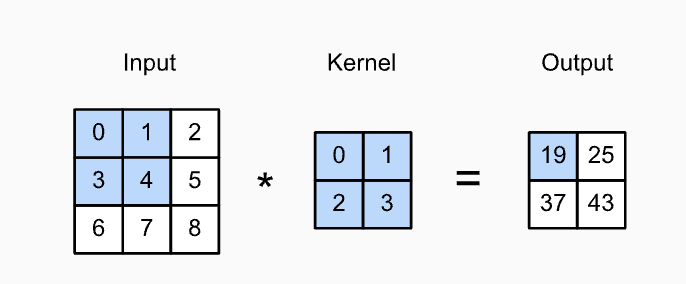
\includegraphics[keepaspectratio]{main_files/image.png}}
Fig. 7.2.1

It is important to note that since kernels in deep learning are learned
from data, the outputs of convolutional layers remain the same whether
the layers perform strict convolution or cross-correlation. For example,
if a convolutional layer learns the kernel \(K\) in Fig. 7.2.1 and
performs strict convolution, flipping the kernel will produce the same
output as the cross-correlation.

We continue to use the term ``convolution'' in the deep learning
context, even though, technically, we refer to cross-correlation. The
term ``element'' refers to any entry of a tensor representing a layer's
output or a convolution kernel.

    \subsubsection*{7.2.6. Feature Map and Receptive
Field}\label{feature-map-and-receptive-field}

    As described in Section 7.1.4, the convolutional layer output in Fig.
7.2.1 is called a feature map. The receptive field of an element \(x\)
in some layer refers to all the elements that affect the calculation of
\(x\), and it may be larger than the input's actual size.

Using Fig. 7.2.1, the receptive field of the shaded output element
(value 19) is the four shaded elements of the input. For a deeper CNN
with another 2 × 2 convolutional layer, the receptive field for an
element \(z\) on \(Y\) includes all input elements, allowing the network
to detect broader features.

The concept of receptive fields originates from neurophysiology,
particularly experiments by Hubel and Wiesel, which found that lower
levels respond to edges and shapes. Field (1987) later showed this
effect on natural images using convolutional kernels, as illustrated in
Fig. 7.2.2. These insights help explain the success of deep learning,
especially in image classification tasks.

    \subsubsection*{7.2.7. Summary}\label{summary}

    The core computation for a convolutional layer is a cross-correlation
operation. With multiple input and output channels, the operation
becomes a matrix--matrix computation between channels. This process is
highly local, allowing for significant hardware optimizations. This
locality allows chip designers to focus on fast computation rather than
memory, enabling more accessible and affordable computer vision
solutions.

Convolutions serve various purposes, such as detecting edges, blurring,
or sharpening images. Importantly, filters do not need to be manually
designed; they can be learned from data, which replaces traditional
feature engineering. These learned filters correspond to receptive
fields and feature maps, not only in neural networks but also in the
brain, providing confidence in the direction of deep learning research.

    \subsubsection*{7.2.8. Exercises}\label{exercises}

    \subsection*{7.3. Padding and Stride}\label{padding-and-stride}

    \begin{tcolorbox}[breakable, size=fbox, boxrule=1pt, pad at break*=1mm,colback=cellbackground, colframe=cellborder]
\prompt{In}{incolor}{11}{\boxspacing}
\begin{Verbatim}[commandchars=\\\{\}]
\PY{k+kn}{import} \PY{n+nn}{torch}
\PY{k+kn}{from} \PY{n+nn}{torch} \PY{k+kn}{import} \PY{n}{nn}
\end{Verbatim}
\end{tcolorbox}

    \subsubsection*{7.3.1. Padding}\label{padding}

    \begin{tcolorbox}[breakable, size=fbox, boxrule=1pt, pad at break*=1mm,colback=cellbackground, colframe=cellborder]
\prompt{In}{incolor}{12}{\boxspacing}
\begin{Verbatim}[commandchars=\\\{\}]
\PY{k}{def} \PY{n+nf}{comp\PYZus{}conv2d}\PY{p}{(}\PY{n}{conv2d}\PY{p}{,} \PY{n}{X}\PY{p}{)}\PY{p}{:}
    \PY{n}{X} \PY{o}{=} \PY{n}{X}\PY{o}{.}\PY{n}{reshape}\PY{p}{(}\PY{p}{(}\PY{l+m+mi}{1}\PY{p}{,} \PY{l+m+mi}{1}\PY{p}{)} \PY{o}{+} \PY{n}{X}\PY{o}{.}\PY{n}{shape}\PY{p}{)}
    \PY{n}{Y} \PY{o}{=} \PY{n}{conv2d}\PY{p}{(}\PY{n}{X}\PY{p}{)}
    \PY{k}{return} \PY{n}{Y}\PY{o}{.}\PY{n}{reshape}\PY{p}{(}\PY{n}{Y}\PY{o}{.}\PY{n}{shape}\PY{p}{[}\PY{l+m+mi}{2}\PY{p}{:}\PY{p}{]}\PY{p}{)}

\PY{n}{conv2d} \PY{o}{=} \PY{n}{nn}\PY{o}{.}\PY{n}{LazyConv2d}\PY{p}{(}\PY{l+m+mi}{1}\PY{p}{,} \PY{n}{kernel\PYZus{}size}\PY{o}{=}\PY{l+m+mi}{3}\PY{p}{,} \PY{n}{padding}\PY{o}{=}\PY{l+m+mi}{1}\PY{p}{)}
\PY{n}{X} \PY{o}{=} \PY{n}{torch}\PY{o}{.}\PY{n}{rand}\PY{p}{(}\PY{n}{size}\PY{o}{=}\PY{p}{(}\PY{l+m+mi}{8}\PY{p}{,} \PY{l+m+mi}{8}\PY{p}{)}\PY{p}{)}
\PY{n}{comp\PYZus{}conv2d}\PY{p}{(}\PY{n}{conv2d}\PY{p}{,} \PY{n}{X}\PY{p}{)}\PY{o}{.}\PY{n}{shape}
\end{Verbatim}
\end{tcolorbox}

            \begin{tcolorbox}[breakable, size=fbox, boxrule=.5pt, pad at break*=1mm, opacityfill=0]
\prompt{Out}{outcolor}{12}{\boxspacing}
\begin{Verbatim}[commandchars=\\\{\}]
torch.Size([8, 8])
\end{Verbatim}
\end{tcolorbox}
        
    \begin{tcolorbox}[breakable, size=fbox, boxrule=1pt, pad at break*=1mm,colback=cellbackground, colframe=cellborder]
\prompt{In}{incolor}{13}{\boxspacing}
\begin{Verbatim}[commandchars=\\\{\}]
\PY{n}{conv2d} \PY{o}{=} \PY{n}{nn}\PY{o}{.}\PY{n}{LazyConv2d}\PY{p}{(}\PY{l+m+mi}{1}\PY{p}{,} \PY{n}{kernel\PYZus{}size}\PY{o}{=}\PY{p}{(}\PY{l+m+mi}{5}\PY{p}{,} \PY{l+m+mi}{3}\PY{p}{)}\PY{p}{,} \PY{n}{padding}\PY{o}{=}\PY{p}{(}\PY{l+m+mi}{2}\PY{p}{,} \PY{l+m+mi}{1}\PY{p}{)}\PY{p}{)}
\PY{n}{comp\PYZus{}conv2d}\PY{p}{(}\PY{n}{conv2d}\PY{p}{,} \PY{n}{X}\PY{p}{)}\PY{o}{.}\PY{n}{shape}
\end{Verbatim}
\end{tcolorbox}

            \begin{tcolorbox}[breakable, size=fbox, boxrule=.5pt, pad at break*=1mm, opacityfill=0]
\prompt{Out}{outcolor}{13}{\boxspacing}
\begin{Verbatim}[commandchars=\\\{\}]
torch.Size([8, 8])
\end{Verbatim}
\end{tcolorbox}
        
    \subsubsection*{7.3.2. Stride}\label{stride}

    \begin{tcolorbox}[breakable, size=fbox, boxrule=1pt, pad at break*=1mm,colback=cellbackground, colframe=cellborder]
\prompt{In}{incolor}{14}{\boxspacing}
\begin{Verbatim}[commandchars=\\\{\}]
\PY{n}{conv2d} \PY{o}{=} \PY{n}{nn}\PY{o}{.}\PY{n}{LazyConv2d}\PY{p}{(}\PY{l+m+mi}{1}\PY{p}{,} \PY{n}{kernel\PYZus{}size}\PY{o}{=}\PY{l+m+mi}{3}\PY{p}{,} \PY{n}{padding}\PY{o}{=}\PY{l+m+mi}{1}\PY{p}{,} \PY{n}{stride}\PY{o}{=}\PY{l+m+mi}{2}\PY{p}{)}
\PY{n}{comp\PYZus{}conv2d}\PY{p}{(}\PY{n}{conv2d}\PY{p}{,} \PY{n}{X}\PY{p}{)}\PY{o}{.}\PY{n}{shape}
\end{Verbatim}
\end{tcolorbox}

            \begin{tcolorbox}[breakable, size=fbox, boxrule=.5pt, pad at break*=1mm, opacityfill=0]
\prompt{Out}{outcolor}{14}{\boxspacing}
\begin{Verbatim}[commandchars=\\\{\}]
torch.Size([4, 4])
\end{Verbatim}
\end{tcolorbox}
        
    \begin{tcolorbox}[breakable, size=fbox, boxrule=1pt, pad at break*=1mm,colback=cellbackground, colframe=cellborder]
\prompt{In}{incolor}{15}{\boxspacing}
\begin{Verbatim}[commandchars=\\\{\}]
\PY{n}{conv2d} \PY{o}{=} \PY{n}{nn}\PY{o}{.}\PY{n}{LazyConv2d}\PY{p}{(}\PY{l+m+mi}{1}\PY{p}{,} \PY{n}{kernel\PYZus{}size}\PY{o}{=}\PY{p}{(}\PY{l+m+mi}{3}\PY{p}{,} \PY{l+m+mi}{5}\PY{p}{)}\PY{p}{,} \PY{n}{padding}\PY{o}{=}\PY{p}{(}\PY{l+m+mi}{0}\PY{p}{,} \PY{l+m+mi}{1}\PY{p}{)}\PY{p}{,} \PY{n}{stride}\PY{o}{=}\PY{p}{(}\PY{l+m+mi}{3}\PY{p}{,} \PY{l+m+mi}{4}\PY{p}{)}\PY{p}{)}
\PY{n}{comp\PYZus{}conv2d}\PY{p}{(}\PY{n}{conv2d}\PY{p}{,} \PY{n}{X}\PY{p}{)}\PY{o}{.}\PY{n}{shape}
\end{Verbatim}
\end{tcolorbox}

            \begin{tcolorbox}[breakable, size=fbox, boxrule=.5pt, pad at break*=1mm, opacityfill=0]
\prompt{Out}{outcolor}{15}{\boxspacing}
\begin{Verbatim}[commandchars=\\\{\}]
torch.Size([2, 2])
\end{Verbatim}
\end{tcolorbox}
        
    \subsubsection*{7.3.3. Summary and
Discussion}\label{summary-and-discussion}

    Padding is used to increase the height and width of the output, ensuring
that the output size remains the same as the input size and that all
pixels are treated equally. Typically, symmetric padding is applied to
both the height and width of the input, referred to as \((p_h, p_w)\),
or simply \(p\) when both are equal.

Strides, represented by \(s_h\) (horizontal) and \(s_w\) (vertical),
similarly affect the output. When strides are equal, we refer to stride
\(s\), which reduces the resolution of the output by a factor of \(1/n\)
for \(n > 1\). By default, padding is set to 0 and stride to 1.

Padding usually adds zeros around the image, which is computationally
efficient. This allows CNNs to implicitly learn positional information
by determining the ``whitespace.'' Various alternatives to zero-padding
exist, but Alsallakh et al.~(2020) reviewed these options without
concluding when nonzero paddings should be used.

    \subsection*{7.4. Multiple Input and Multiple Output
Channels}\label{multiple-input-and-multiple-output-channels}

    \begin{tcolorbox}[breakable, size=fbox, boxrule=1pt, pad at break*=1mm,colback=cellbackground, colframe=cellborder]
\prompt{In}{incolor}{16}{\boxspacing}
\begin{Verbatim}[commandchars=\\\{\}]
\PY{k+kn}{import} \PY{n+nn}{torch}
\PY{k+kn}{from} \PY{n+nn}{d2l} \PY{k+kn}{import} \PY{n}{torch} \PY{k}{as} \PY{n}{d2l}
\end{Verbatim}
\end{tcolorbox}

    \subsubsection*{7.4.1. Multiple Input
Channels}\label{multiple-input-channels}

    \begin{tcolorbox}[breakable, size=fbox, boxrule=1pt, pad at break*=1mm,colback=cellbackground, colframe=cellborder]
\prompt{In}{incolor}{17}{\boxspacing}
\begin{Verbatim}[commandchars=\\\{\}]
\PY{k}{def} \PY{n+nf}{corr2d\PYZus{}multi\PYZus{}in}\PY{p}{(}\PY{n}{X}\PY{p}{,} \PY{n}{K}\PY{p}{)}\PY{p}{:}
    \PY{k}{return} \PY{n+nb}{sum}\PY{p}{(}\PY{n}{d2l}\PY{o}{.}\PY{n}{corr2d}\PY{p}{(}\PY{n}{x}\PY{p}{,} \PY{n}{k}\PY{p}{)} \PY{k}{for} \PY{n}{x}\PY{p}{,} \PY{n}{k} \PY{o+ow}{in} \PY{n+nb}{zip}\PY{p}{(}\PY{n}{X}\PY{p}{,} \PY{n}{K}\PY{p}{)}\PY{p}{)}
\end{Verbatim}
\end{tcolorbox}

    \begin{tcolorbox}[breakable, size=fbox, boxrule=1pt, pad at break*=1mm,colback=cellbackground, colframe=cellborder]
\prompt{In}{incolor}{18}{\boxspacing}
\begin{Verbatim}[commandchars=\\\{\}]
\PY{n}{X} \PY{o}{=} \PY{n}{torch}\PY{o}{.}\PY{n}{tensor}\PY{p}{(}\PY{p}{[}\PY{p}{[}\PY{p}{[}\PY{l+m+mf}{0.0}\PY{p}{,} \PY{l+m+mf}{1.0}\PY{p}{,} \PY{l+m+mf}{2.0}\PY{p}{]}\PY{p}{,} \PY{p}{[}\PY{l+m+mf}{3.0}\PY{p}{,} \PY{l+m+mf}{4.0}\PY{p}{,} \PY{l+m+mf}{5.0}\PY{p}{]}\PY{p}{,} \PY{p}{[}\PY{l+m+mf}{6.0}\PY{p}{,} \PY{l+m+mf}{7.0}\PY{p}{,} \PY{l+m+mf}{8.0}\PY{p}{]}\PY{p}{]}\PY{p}{,}
               \PY{p}{[}\PY{p}{[}\PY{l+m+mf}{1.0}\PY{p}{,} \PY{l+m+mf}{2.0}\PY{p}{,} \PY{l+m+mf}{3.0}\PY{p}{]}\PY{p}{,} \PY{p}{[}\PY{l+m+mf}{4.0}\PY{p}{,} \PY{l+m+mf}{5.0}\PY{p}{,} \PY{l+m+mf}{6.0}\PY{p}{]}\PY{p}{,} \PY{p}{[}\PY{l+m+mf}{7.0}\PY{p}{,} \PY{l+m+mf}{8.0}\PY{p}{,} \PY{l+m+mf}{9.0}\PY{p}{]}\PY{p}{]}\PY{p}{]}\PY{p}{)}
\PY{n}{K} \PY{o}{=} \PY{n}{torch}\PY{o}{.}\PY{n}{tensor}\PY{p}{(}\PY{p}{[}\PY{p}{[}\PY{p}{[}\PY{l+m+mf}{0.0}\PY{p}{,} \PY{l+m+mf}{1.0}\PY{p}{]}\PY{p}{,} \PY{p}{[}\PY{l+m+mf}{2.0}\PY{p}{,} \PY{l+m+mf}{3.0}\PY{p}{]}\PY{p}{]}\PY{p}{,} \PY{p}{[}\PY{p}{[}\PY{l+m+mf}{1.0}\PY{p}{,} \PY{l+m+mf}{2.0}\PY{p}{]}\PY{p}{,} \PY{p}{[}\PY{l+m+mf}{3.0}\PY{p}{,} \PY{l+m+mf}{4.0}\PY{p}{]}\PY{p}{]}\PY{p}{]}\PY{p}{)}

\PY{n}{corr2d\PYZus{}multi\PYZus{}in}\PY{p}{(}\PY{n}{X}\PY{p}{,} \PY{n}{K}\PY{p}{)}
\end{Verbatim}
\end{tcolorbox}

            \begin{tcolorbox}[breakable, size=fbox, boxrule=.5pt, pad at break*=1mm, opacityfill=0]
\prompt{Out}{outcolor}{18}{\boxspacing}
\begin{Verbatim}[commandchars=\\\{\}]
tensor([[ 56.,  72.],
        [104., 120.]])
\end{Verbatim}
\end{tcolorbox}
        
    \subsubsection*{7.4.2. Multiple Output
Channels}\label{multiple-output-channels}

    \begin{tcolorbox}[breakable, size=fbox, boxrule=1pt, pad at break*=1mm,colback=cellbackground, colframe=cellborder]
\prompt{In}{incolor}{19}{\boxspacing}
\begin{Verbatim}[commandchars=\\\{\}]
\PY{k}{def} \PY{n+nf}{corr2d\PYZus{}multi\PYZus{}in\PYZus{}out}\PY{p}{(}\PY{n}{X}\PY{p}{,} \PY{n}{K}\PY{p}{)}\PY{p}{:}
    \PY{k}{return} \PY{n}{torch}\PY{o}{.}\PY{n}{stack}\PY{p}{(}\PY{p}{[}\PY{n}{corr2d\PYZus{}multi\PYZus{}in}\PY{p}{(}\PY{n}{X}\PY{p}{,} \PY{n}{k}\PY{p}{)} \PY{k}{for} \PY{n}{k} \PY{o+ow}{in} \PY{n}{K}\PY{p}{]}\PY{p}{,} \PY{l+m+mi}{0}\PY{p}{)}
\end{Verbatim}
\end{tcolorbox}

    \begin{tcolorbox}[breakable, size=fbox, boxrule=1pt, pad at break*=1mm,colback=cellbackground, colframe=cellborder]
\prompt{In}{incolor}{20}{\boxspacing}
\begin{Verbatim}[commandchars=\\\{\}]
\PY{n}{K} \PY{o}{=} \PY{n}{torch}\PY{o}{.}\PY{n}{stack}\PY{p}{(}\PY{p}{(}\PY{n}{K}\PY{p}{,} \PY{n}{K} \PY{o}{+} \PY{l+m+mi}{1}\PY{p}{,} \PY{n}{K} \PY{o}{+} \PY{l+m+mi}{2}\PY{p}{)}\PY{p}{,} \PY{l+m+mi}{0}\PY{p}{)}
\PY{n}{K}\PY{o}{.}\PY{n}{shape}
\end{Verbatim}
\end{tcolorbox}

            \begin{tcolorbox}[breakable, size=fbox, boxrule=.5pt, pad at break*=1mm, opacityfill=0]
\prompt{Out}{outcolor}{20}{\boxspacing}
\begin{Verbatim}[commandchars=\\\{\}]
torch.Size([3, 2, 2, 2])
\end{Verbatim}
\end{tcolorbox}
        
    \begin{tcolorbox}[breakable, size=fbox, boxrule=1pt, pad at break*=1mm,colback=cellbackground, colframe=cellborder]
\prompt{In}{incolor}{21}{\boxspacing}
\begin{Verbatim}[commandchars=\\\{\}]
\PY{n}{corr2d\PYZus{}multi\PYZus{}in\PYZus{}out}\PY{p}{(}\PY{n}{X}\PY{p}{,} \PY{n}{K}\PY{p}{)}
\end{Verbatim}
\end{tcolorbox}

            \begin{tcolorbox}[breakable, size=fbox, boxrule=.5pt, pad at break*=1mm, opacityfill=0]
\prompt{Out}{outcolor}{21}{\boxspacing}
\begin{Verbatim}[commandchars=\\\{\}]
tensor([[[ 56.,  72.],
         [104., 120.]],

        [[ 76., 100.],
         [148., 172.]],

        [[ 96., 128.],
         [192., 224.]]])
\end{Verbatim}
\end{tcolorbox}
        
    \subsubsection*{\texorpdfstring{7.4.3. \(1 \times 1\) Convolutional
Layer}{7.4.3. 1 \textbackslash times 1 Convolutional Layer}}\label{times-1-convolutional-layer}

    \begin{tcolorbox}[breakable, size=fbox, boxrule=1pt, pad at break*=1mm,colback=cellbackground, colframe=cellborder]
\prompt{In}{incolor}{22}{\boxspacing}
\begin{Verbatim}[commandchars=\\\{\}]
\PY{k}{def} \PY{n+nf}{corr2d\PYZus{}multi\PYZus{}in\PYZus{}out\PYZus{}1x1}\PY{p}{(}\PY{n}{X}\PY{p}{,} \PY{n}{K}\PY{p}{)}\PY{p}{:}
    \PY{n}{c\PYZus{}i}\PY{p}{,} \PY{n}{h}\PY{p}{,} \PY{n}{w} \PY{o}{=} \PY{n}{X}\PY{o}{.}\PY{n}{shape}
    \PY{n}{c\PYZus{}o} \PY{o}{=} \PY{n}{K}\PY{o}{.}\PY{n}{shape}\PY{p}{[}\PY{l+m+mi}{0}\PY{p}{]}
    \PY{n}{X} \PY{o}{=} \PY{n}{X}\PY{o}{.}\PY{n}{reshape}\PY{p}{(}\PY{p}{(}\PY{n}{c\PYZus{}i}\PY{p}{,} \PY{n}{h} \PY{o}{*} \PY{n}{w}\PY{p}{)}\PY{p}{)}
    \PY{n}{K} \PY{o}{=} \PY{n}{K}\PY{o}{.}\PY{n}{reshape}\PY{p}{(}\PY{p}{(}\PY{n}{c\PYZus{}o}\PY{p}{,} \PY{n}{c\PYZus{}i}\PY{p}{)}\PY{p}{)}
    \PY{n}{Y} \PY{o}{=} \PY{n}{torch}\PY{o}{.}\PY{n}{matmul}\PY{p}{(}\PY{n}{K}\PY{p}{,} \PY{n}{X}\PY{p}{)}
    \PY{k}{return} \PY{n}{Y}\PY{o}{.}\PY{n}{reshape}\PY{p}{(}\PY{p}{(}\PY{n}{c\PYZus{}o}\PY{p}{,} \PY{n}{h}\PY{p}{,} \PY{n}{w}\PY{p}{)}\PY{p}{)}
\end{Verbatim}
\end{tcolorbox}

    \begin{tcolorbox}[breakable, size=fbox, boxrule=1pt, pad at break*=1mm,colback=cellbackground, colframe=cellborder]
\prompt{In}{incolor}{23}{\boxspacing}
\begin{Verbatim}[commandchars=\\\{\}]
\PY{n}{X} \PY{o}{=} \PY{n}{torch}\PY{o}{.}\PY{n}{normal}\PY{p}{(}\PY{l+m+mi}{0}\PY{p}{,} \PY{l+m+mi}{1}\PY{p}{,} \PY{p}{(}\PY{l+m+mi}{3}\PY{p}{,} \PY{l+m+mi}{3}\PY{p}{,} \PY{l+m+mi}{3}\PY{p}{)}\PY{p}{)}
\PY{n}{K} \PY{o}{=} \PY{n}{torch}\PY{o}{.}\PY{n}{normal}\PY{p}{(}\PY{l+m+mi}{0}\PY{p}{,} \PY{l+m+mi}{1}\PY{p}{,} \PY{p}{(}\PY{l+m+mi}{2}\PY{p}{,} \PY{l+m+mi}{3}\PY{p}{,} \PY{l+m+mi}{1}\PY{p}{,} \PY{l+m+mi}{1}\PY{p}{)}\PY{p}{)}
\PY{n}{Y1} \PY{o}{=} \PY{n}{corr2d\PYZus{}multi\PYZus{}in\PYZus{}out\PYZus{}1x1}\PY{p}{(}\PY{n}{X}\PY{p}{,} \PY{n}{K}\PY{p}{)}
\PY{n}{Y2} \PY{o}{=} \PY{n}{corr2d\PYZus{}multi\PYZus{}in\PYZus{}out}\PY{p}{(}\PY{n}{X}\PY{p}{,} \PY{n}{K}\PY{p}{)}
\PY{k}{assert} \PY{n+nb}{float}\PY{p}{(}\PY{n}{torch}\PY{o}{.}\PY{n}{abs}\PY{p}{(}\PY{n}{Y1} \PY{o}{\PYZhy{}} \PY{n}{Y2}\PY{p}{)}\PY{o}{.}\PY{n}{sum}\PY{p}{(}\PY{p}{)}\PY{p}{)} \PY{o}{\PYZlt{}} \PY{l+m+mf}{1e\PYZhy{}6}
\end{Verbatim}
\end{tcolorbox}

    \subsubsection*{7.4.4. Discussion}\label{discussion}

    Channels enable us to combine the advantages of MLPs, which introduce
significant nonlinearities, and convolutions, which allow localized
feature analysis. Channels allow CNNs to process multiple features, such
as edge and shape detectors, simultaneously. They offer a practical
trade-off between reducing parameters, thanks to translation invariance
and locality, and the need for expressive, diverse models.

However, this flexibility comes with a cost. For an image of size
\(h \times w\), the computational cost of a \(k \times k\) convolution
is \(O(h \cdot w \cdot k^2)\). For \(c_i\) input channels and \(c_o\)
output channels, the cost increases to
\(O(h \cdot w \cdot k^2 \cdot c_i \cdot c_o)\). For example, a
\(256 × 256\) pixel image with a \(5 × 5\) kernel and 128 input and
output channels results in over 53 billion operations. Methods like
block-diagonal operations, as used in architectures such as ResNeXt (Xie
et al., 2017), are introduced to reduce this computational burden.

    

    \subsection*{7.5. Pooling}\label{pooling}

    \begin{tcolorbox}[breakable, size=fbox, boxrule=1pt, pad at break*=1mm,colback=cellbackground, colframe=cellborder]
\prompt{In}{incolor}{24}{\boxspacing}
\begin{Verbatim}[commandchars=\\\{\}]
\PY{k+kn}{import} \PY{n+nn}{torch}
\PY{k+kn}{from} \PY{n+nn}{torch} \PY{k+kn}{import} \PY{n}{nn}
\PY{k+kn}{from} \PY{n+nn}{d2l} \PY{k+kn}{import} \PY{n}{torch} \PY{k}{as} \PY{n}{d2l}
\end{Verbatim}
\end{tcolorbox}

    \subsubsection*{7.5.1. Maximum Pooling and Average
Pooling}\label{maximum-pooling-and-average-pooling}

    \begin{tcolorbox}[breakable, size=fbox, boxrule=1pt, pad at break*=1mm,colback=cellbackground, colframe=cellborder]
\prompt{In}{incolor}{25}{\boxspacing}
\begin{Verbatim}[commandchars=\\\{\}]
\PY{k}{def} \PY{n+nf}{pool2d}\PY{p}{(}\PY{n}{X}\PY{p}{,} \PY{n}{pool\PYZus{}size}\PY{p}{,} \PY{n}{mode}\PY{o}{=}\PY{l+s+s1}{\PYZsq{}}\PY{l+s+s1}{max}\PY{l+s+s1}{\PYZsq{}}\PY{p}{)}\PY{p}{:}
    \PY{n}{p\PYZus{}h}\PY{p}{,} \PY{n}{p\PYZus{}w} \PY{o}{=} \PY{n}{pool\PYZus{}size}
    \PY{n}{Y} \PY{o}{=} \PY{n}{torch}\PY{o}{.}\PY{n}{zeros}\PY{p}{(}\PY{p}{(}\PY{n}{X}\PY{o}{.}\PY{n}{shape}\PY{p}{[}\PY{l+m+mi}{0}\PY{p}{]} \PY{o}{\PYZhy{}} \PY{n}{p\PYZus{}h} \PY{o}{+} \PY{l+m+mi}{1}\PY{p}{,} \PY{n}{X}\PY{o}{.}\PY{n}{shape}\PY{p}{[}\PY{l+m+mi}{1}\PY{p}{]} \PY{o}{\PYZhy{}} \PY{n}{p\PYZus{}w} \PY{o}{+} \PY{l+m+mi}{1}\PY{p}{)}\PY{p}{)}
    \PY{k}{for} \PY{n}{i} \PY{o+ow}{in} \PY{n+nb}{range}\PY{p}{(}\PY{n}{Y}\PY{o}{.}\PY{n}{shape}\PY{p}{[}\PY{l+m+mi}{0}\PY{p}{]}\PY{p}{)}\PY{p}{:}
        \PY{k}{for} \PY{n}{j} \PY{o+ow}{in} \PY{n+nb}{range}\PY{p}{(}\PY{n}{Y}\PY{o}{.}\PY{n}{shape}\PY{p}{[}\PY{l+m+mi}{1}\PY{p}{]}\PY{p}{)}\PY{p}{:}
            \PY{k}{if} \PY{n}{mode} \PY{o}{==} \PY{l+s+s1}{\PYZsq{}}\PY{l+s+s1}{max}\PY{l+s+s1}{\PYZsq{}}\PY{p}{:}
                \PY{n}{Y}\PY{p}{[}\PY{n}{i}\PY{p}{,} \PY{n}{j}\PY{p}{]} \PY{o}{=} \PY{n}{X}\PY{p}{[}\PY{n}{i}\PY{p}{:} \PY{n}{i} \PY{o}{+} \PY{n}{p\PYZus{}h}\PY{p}{,} \PY{n}{j}\PY{p}{:} \PY{n}{j} \PY{o}{+} \PY{n}{p\PYZus{}w}\PY{p}{]}\PY{o}{.}\PY{n}{max}\PY{p}{(}\PY{p}{)}
            \PY{k}{elif} \PY{n}{mode} \PY{o}{==} \PY{l+s+s1}{\PYZsq{}}\PY{l+s+s1}{avg}\PY{l+s+s1}{\PYZsq{}}\PY{p}{:}
                \PY{n}{Y}\PY{p}{[}\PY{n}{i}\PY{p}{,} \PY{n}{j}\PY{p}{]} \PY{o}{=} \PY{n}{X}\PY{p}{[}\PY{n}{i}\PY{p}{:} \PY{n}{i} \PY{o}{+} \PY{n}{p\PYZus{}h}\PY{p}{,} \PY{n}{j}\PY{p}{:} \PY{n}{j} \PY{o}{+} \PY{n}{p\PYZus{}w}\PY{p}{]}\PY{o}{.}\PY{n}{mean}\PY{p}{(}\PY{p}{)}
    \PY{k}{return} \PY{n}{Y}
\end{Verbatim}
\end{tcolorbox}

    \begin{tcolorbox}[breakable, size=fbox, boxrule=1pt, pad at break*=1mm,colback=cellbackground, colframe=cellborder]
\prompt{In}{incolor}{26}{\boxspacing}
\begin{Verbatim}[commandchars=\\\{\}]
\PY{n}{X} \PY{o}{=} \PY{n}{torch}\PY{o}{.}\PY{n}{tensor}\PY{p}{(}\PY{p}{[}\PY{p}{[}\PY{l+m+mf}{0.0}\PY{p}{,} \PY{l+m+mf}{1.0}\PY{p}{,} \PY{l+m+mf}{2.0}\PY{p}{]}\PY{p}{,} \PY{p}{[}\PY{l+m+mf}{3.0}\PY{p}{,} \PY{l+m+mf}{4.0}\PY{p}{,} \PY{l+m+mf}{5.0}\PY{p}{]}\PY{p}{,} \PY{p}{[}\PY{l+m+mf}{6.0}\PY{p}{,} \PY{l+m+mf}{7.0}\PY{p}{,} \PY{l+m+mf}{8.0}\PY{p}{]}\PY{p}{]}\PY{p}{)}
\PY{n}{pool2d}\PY{p}{(}\PY{n}{X}\PY{p}{,} \PY{p}{(}\PY{l+m+mi}{2}\PY{p}{,} \PY{l+m+mi}{2}\PY{p}{)}\PY{p}{)}
\end{Verbatim}
\end{tcolorbox}

            \begin{tcolorbox}[breakable, size=fbox, boxrule=.5pt, pad at break*=1mm, opacityfill=0]
\prompt{Out}{outcolor}{26}{\boxspacing}
\begin{Verbatim}[commandchars=\\\{\}]
tensor([[4., 5.],
        [7., 8.]])
\end{Verbatim}
\end{tcolorbox}
        
    \begin{tcolorbox}[breakable, size=fbox, boxrule=1pt, pad at break*=1mm,colback=cellbackground, colframe=cellborder]
\prompt{In}{incolor}{27}{\boxspacing}
\begin{Verbatim}[commandchars=\\\{\}]
\PY{n}{pool2d}\PY{p}{(}\PY{n}{X}\PY{p}{,} \PY{p}{(}\PY{l+m+mi}{2}\PY{p}{,} \PY{l+m+mi}{2}\PY{p}{)}\PY{p}{,} \PY{l+s+s1}{\PYZsq{}}\PY{l+s+s1}{avg}\PY{l+s+s1}{\PYZsq{}}\PY{p}{)}
\end{Verbatim}
\end{tcolorbox}

            \begin{tcolorbox}[breakable, size=fbox, boxrule=.5pt, pad at break*=1mm, opacityfill=0]
\prompt{Out}{outcolor}{27}{\boxspacing}
\begin{Verbatim}[commandchars=\\\{\}]
tensor([[2., 3.],
        [5., 6.]])
\end{Verbatim}
\end{tcolorbox}
        
    \subsubsection*{7.5.2. Padding and Stride}\label{padding-and-stride}

    \begin{tcolorbox}[breakable, size=fbox, boxrule=1pt, pad at break*=1mm,colback=cellbackground, colframe=cellborder]
\prompt{In}{incolor}{28}{\boxspacing}
\begin{Verbatim}[commandchars=\\\{\}]
\PY{n}{X} \PY{o}{=} \PY{n}{torch}\PY{o}{.}\PY{n}{arange}\PY{p}{(}\PY{l+m+mi}{16}\PY{p}{,} \PY{n}{dtype}\PY{o}{=}\PY{n}{torch}\PY{o}{.}\PY{n}{float32}\PY{p}{)}\PY{o}{.}\PY{n}{reshape}\PY{p}{(}\PY{p}{(}\PY{l+m+mi}{1}\PY{p}{,} \PY{l+m+mi}{1}\PY{p}{,} \PY{l+m+mi}{4}\PY{p}{,} \PY{l+m+mi}{4}\PY{p}{)}\PY{p}{)}
\PY{n}{X}
\end{Verbatim}
\end{tcolorbox}

            \begin{tcolorbox}[breakable, size=fbox, boxrule=.5pt, pad at break*=1mm, opacityfill=0]
\prompt{Out}{outcolor}{28}{\boxspacing}
\begin{Verbatim}[commandchars=\\\{\}]
tensor([[[[ 0.,  1.,  2.,  3.],
          [ 4.,  5.,  6.,  7.],
          [ 8.,  9., 10., 11.],
          [12., 13., 14., 15.]]]])
\end{Verbatim}
\end{tcolorbox}
        
    \begin{tcolorbox}[breakable, size=fbox, boxrule=1pt, pad at break*=1mm,colback=cellbackground, colframe=cellborder]
\prompt{In}{incolor}{29}{\boxspacing}
\begin{Verbatim}[commandchars=\\\{\}]
\PY{n}{pool2d} \PY{o}{=} \PY{n}{nn}\PY{o}{.}\PY{n}{MaxPool2d}\PY{p}{(}\PY{l+m+mi}{3}\PY{p}{)}
\PY{n}{pool2d}\PY{p}{(}\PY{n}{X}\PY{p}{)}
\end{Verbatim}
\end{tcolorbox}

            \begin{tcolorbox}[breakable, size=fbox, boxrule=.5pt, pad at break*=1mm, opacityfill=0]
\prompt{Out}{outcolor}{29}{\boxspacing}
\begin{Verbatim}[commandchars=\\\{\}]
tensor([[[[10.]]]])
\end{Verbatim}
\end{tcolorbox}
        
    \begin{tcolorbox}[breakable, size=fbox, boxrule=1pt, pad at break*=1mm,colback=cellbackground, colframe=cellborder]
\prompt{In}{incolor}{30}{\boxspacing}
\begin{Verbatim}[commandchars=\\\{\}]
\PY{n}{pool2d} \PY{o}{=} \PY{n}{nn}\PY{o}{.}\PY{n}{MaxPool2d}\PY{p}{(}\PY{l+m+mi}{3}\PY{p}{,} \PY{n}{padding}\PY{o}{=}\PY{l+m+mi}{1}\PY{p}{,} \PY{n}{stride}\PY{o}{=}\PY{l+m+mi}{2}\PY{p}{)}
\PY{n}{pool2d}\PY{p}{(}\PY{n}{X}\PY{p}{)}
\end{Verbatim}
\end{tcolorbox}

            \begin{tcolorbox}[breakable, size=fbox, boxrule=.5pt, pad at break*=1mm, opacityfill=0]
\prompt{Out}{outcolor}{30}{\boxspacing}
\begin{Verbatim}[commandchars=\\\{\}]
tensor([[[[ 5.,  7.],
          [13., 15.]]]])
\end{Verbatim}
\end{tcolorbox}
        
    \begin{tcolorbox}[breakable, size=fbox, boxrule=1pt, pad at break*=1mm,colback=cellbackground, colframe=cellborder]
\prompt{In}{incolor}{31}{\boxspacing}
\begin{Verbatim}[commandchars=\\\{\}]
\PY{n}{pool2d} \PY{o}{=} \PY{n}{nn}\PY{o}{.}\PY{n}{MaxPool2d}\PY{p}{(}\PY{p}{(}\PY{l+m+mi}{2}\PY{p}{,} \PY{l+m+mi}{3}\PY{p}{)}\PY{p}{,} \PY{n}{stride}\PY{o}{=}\PY{p}{(}\PY{l+m+mi}{2}\PY{p}{,} \PY{l+m+mi}{3}\PY{p}{)}\PY{p}{,} \PY{n}{padding}\PY{o}{=}\PY{p}{(}\PY{l+m+mi}{0}\PY{p}{,} \PY{l+m+mi}{1}\PY{p}{)}\PY{p}{)}
\PY{n}{pool2d}\PY{p}{(}\PY{n}{X}\PY{p}{)}
\end{Verbatim}
\end{tcolorbox}

            \begin{tcolorbox}[breakable, size=fbox, boxrule=.5pt, pad at break*=1mm, opacityfill=0]
\prompt{Out}{outcolor}{31}{\boxspacing}
\begin{Verbatim}[commandchars=\\\{\}]
tensor([[[[ 5.,  7.],
          [13., 15.]]]])
\end{Verbatim}
\end{tcolorbox}
        
    \subsubsection*{7.5.3. Multiple Channels}\label{multiple-channels}

    \begin{tcolorbox}[breakable, size=fbox, boxrule=1pt, pad at break*=1mm,colback=cellbackground, colframe=cellborder]
\prompt{In}{incolor}{32}{\boxspacing}
\begin{Verbatim}[commandchars=\\\{\}]
\PY{n}{X} \PY{o}{=} \PY{n}{torch}\PY{o}{.}\PY{n}{cat}\PY{p}{(}\PY{p}{(}\PY{n}{X}\PY{p}{,} \PY{n}{X} \PY{o}{+} \PY{l+m+mi}{1}\PY{p}{)}\PY{p}{,} \PY{l+m+mi}{1}\PY{p}{)}
\PY{n}{X}
\end{Verbatim}
\end{tcolorbox}

            \begin{tcolorbox}[breakable, size=fbox, boxrule=.5pt, pad at break*=1mm, opacityfill=0]
\prompt{Out}{outcolor}{32}{\boxspacing}
\begin{Verbatim}[commandchars=\\\{\}]
tensor([[[[ 0.,  1.,  2.,  3.],
          [ 4.,  5.,  6.,  7.],
          [ 8.,  9., 10., 11.],
          [12., 13., 14., 15.]],

         [[ 1.,  2.,  3.,  4.],
          [ 5.,  6.,  7.,  8.],
          [ 9., 10., 11., 12.],
          [13., 14., 15., 16.]]]])
\end{Verbatim}
\end{tcolorbox}
        
    \begin{tcolorbox}[breakable, size=fbox, boxrule=1pt, pad at break*=1mm,colback=cellbackground, colframe=cellborder]
\prompt{In}{incolor}{33}{\boxspacing}
\begin{Verbatim}[commandchars=\\\{\}]
\PY{n}{pool2d} \PY{o}{=} \PY{n}{nn}\PY{o}{.}\PY{n}{MaxPool2d}\PY{p}{(}\PY{l+m+mi}{3}\PY{p}{,} \PY{n}{padding}\PY{o}{=}\PY{l+m+mi}{1}\PY{p}{,} \PY{n}{stride}\PY{o}{=}\PY{l+m+mi}{2}\PY{p}{)}
\PY{n}{pool2d}\PY{p}{(}\PY{n}{X}\PY{p}{)}
\end{Verbatim}
\end{tcolorbox}

            \begin{tcolorbox}[breakable, size=fbox, boxrule=.5pt, pad at break*=1mm, opacityfill=0]
\prompt{Out}{outcolor}{33}{\boxspacing}
\begin{Verbatim}[commandchars=\\\{\}]
tensor([[[[ 5.,  7.],
          [13., 15.]],

         [[ 6.,  8.],
          [14., 16.]]]])
\end{Verbatim}
\end{tcolorbox}
        
    \subsubsection*{7.5.4. Summary}\label{summary}

    Pooling is a simple operation that aggregates values over a window, such
as \(2 \times 2\). It applies equally to all channels without changing
the number of channels and operates independently on each channel. Among
popular pooling methods, max-pooling is preferred over average pooling
due to its ability to preserve invariance in the output.

Other methods of reducing resolution include stochastic pooling (Zeiler
and Fergus, 2013), which introduces randomization, and fractional
max-pooling (Graham, 2014), which can slightly improve accuracy. Future
sections will introduce more sophisticated aggregation methods, such as
attention mechanisms, that align outputs based on query and
representation vectors.

    \subsection*{7.6. Convolutional Neural Networks
(LeNet)}\label{convolutional-neural-networks-lenet}

    \begin{tcolorbox}[breakable, size=fbox, boxrule=1pt, pad at break*=1mm,colback=cellbackground, colframe=cellborder]
\prompt{In}{incolor}{34}{\boxspacing}
\begin{Verbatim}[commandchars=\\\{\}]
\PY{k+kn}{import} \PY{n+nn}{torch}
\PY{k+kn}{from} \PY{n+nn}{torch} \PY{k+kn}{import} \PY{n}{nn}
\PY{k+kn}{from} \PY{n+nn}{d2l} \PY{k+kn}{import} \PY{n}{torch} \PY{k}{as} \PY{n}{d2l}
\end{Verbatim}
\end{tcolorbox}

    \subsubsection*{7.6.1. LeNet}\label{lenet}

    \begin{tcolorbox}[breakable, size=fbox, boxrule=1pt, pad at break*=1mm,colback=cellbackground, colframe=cellborder]
\prompt{In}{incolor}{35}{\boxspacing}
\begin{Verbatim}[commandchars=\\\{\}]
\PY{k}{def} \PY{n+nf}{init\PYZus{}cnn}\PY{p}{(}\PY{n}{module}\PY{p}{)}\PY{p}{:}
    \PY{k}{if} \PY{n+nb}{type}\PY{p}{(}\PY{n}{module}\PY{p}{)} \PY{o}{==} \PY{n}{nn}\PY{o}{.}\PY{n}{Linear} \PY{o+ow}{or} \PY{n+nb}{type}\PY{p}{(}\PY{n}{module}\PY{p}{)} \PY{o}{==} \PY{n}{nn}\PY{o}{.}\PY{n}{Conv2d}\PY{p}{:}
        \PY{n}{nn}\PY{o}{.}\PY{n}{init}\PY{o}{.}\PY{n}{xavier\PYZus{}uniform\PYZus{}}\PY{p}{(}\PY{n}{module}\PY{o}{.}\PY{n}{weight}\PY{p}{)}

\PY{k}{class} \PY{n+nc}{LeNet}\PY{p}{(}\PY{n}{d2l}\PY{o}{.}\PY{n}{Classifier}\PY{p}{)}\PY{p}{:}
    \PY{k}{def} \PY{n+nf+fm}{\PYZus{}\PYZus{}init\PYZus{}\PYZus{}}\PY{p}{(}\PY{n+nb+bp}{self}\PY{p}{,} \PY{n}{lr}\PY{o}{=}\PY{l+m+mf}{0.1}\PY{p}{,} \PY{n}{num\PYZus{}classes}\PY{o}{=}\PY{l+m+mi}{10}\PY{p}{)}\PY{p}{:}
        \PY{n+nb}{super}\PY{p}{(}\PY{p}{)}\PY{o}{.}\PY{n+nf+fm}{\PYZus{}\PYZus{}init\PYZus{}\PYZus{}}\PY{p}{(}\PY{p}{)}
        \PY{n+nb+bp}{self}\PY{o}{.}\PY{n}{save\PYZus{}hyperparameters}\PY{p}{(}\PY{p}{)}
        \PY{n+nb+bp}{self}\PY{o}{.}\PY{n}{net} \PY{o}{=} \PY{n}{nn}\PY{o}{.}\PY{n}{Sequential}\PY{p}{(}
            \PY{n}{nn}\PY{o}{.}\PY{n}{LazyConv2d}\PY{p}{(}\PY{l+m+mi}{6}\PY{p}{,} \PY{n}{kernel\PYZus{}size}\PY{o}{=}\PY{l+m+mi}{5}\PY{p}{,} \PY{n}{padding}\PY{o}{=}\PY{l+m+mi}{2}\PY{p}{)}\PY{p}{,} \PY{n}{nn}\PY{o}{.}\PY{n}{Sigmoid}\PY{p}{(}\PY{p}{)}\PY{p}{,}
            \PY{n}{nn}\PY{o}{.}\PY{n}{AvgPool2d}\PY{p}{(}\PY{n}{kernel\PYZus{}size}\PY{o}{=}\PY{l+m+mi}{2}\PY{p}{,} \PY{n}{stride}\PY{o}{=}\PY{l+m+mi}{2}\PY{p}{)}\PY{p}{,}
            \PY{n}{nn}\PY{o}{.}\PY{n}{LazyConv2d}\PY{p}{(}\PY{l+m+mi}{16}\PY{p}{,} \PY{n}{kernel\PYZus{}size}\PY{o}{=}\PY{l+m+mi}{5}\PY{p}{)}\PY{p}{,} \PY{n}{nn}\PY{o}{.}\PY{n}{Sigmoid}\PY{p}{(}\PY{p}{)}\PY{p}{,}
            \PY{n}{nn}\PY{o}{.}\PY{n}{AvgPool2d}\PY{p}{(}\PY{n}{kernel\PYZus{}size}\PY{o}{=}\PY{l+m+mi}{2}\PY{p}{,} \PY{n}{stride}\PY{o}{=}\PY{l+m+mi}{2}\PY{p}{)}\PY{p}{,}
            \PY{n}{nn}\PY{o}{.}\PY{n}{Flatten}\PY{p}{(}\PY{p}{)}\PY{p}{,}
            \PY{n}{nn}\PY{o}{.}\PY{n}{LazyLinear}\PY{p}{(}\PY{l+m+mi}{120}\PY{p}{)}\PY{p}{,} \PY{n}{nn}\PY{o}{.}\PY{n}{Sigmoid}\PY{p}{(}\PY{p}{)}\PY{p}{,}
            \PY{n}{nn}\PY{o}{.}\PY{n}{LazyLinear}\PY{p}{(}\PY{l+m+mi}{84}\PY{p}{)}\PY{p}{,} \PY{n}{nn}\PY{o}{.}\PY{n}{Sigmoid}\PY{p}{(}\PY{p}{)}\PY{p}{,}
            \PY{n}{nn}\PY{o}{.}\PY{n}{LazyLinear}\PY{p}{(}\PY{n}{num\PYZus{}classes}\PY{p}{)}\PY{p}{)}
\end{Verbatim}
\end{tcolorbox}

    \begin{tcolorbox}[breakable, size=fbox, boxrule=1pt, pad at break*=1mm,colback=cellbackground, colframe=cellborder]
\prompt{In}{incolor}{36}{\boxspacing}
\begin{Verbatim}[commandchars=\\\{\}]
\PY{n+nd}{@d2l}\PY{o}{.}\PY{n}{add\PYZus{}to\PYZus{}class}\PY{p}{(}\PY{n}{d2l}\PY{o}{.}\PY{n}{Classifier}\PY{p}{)}
\PY{k}{def} \PY{n+nf}{layer\PYZus{}summary}\PY{p}{(}\PY{n+nb+bp}{self}\PY{p}{,} \PY{n}{X\PYZus{}shape}\PY{p}{)}\PY{p}{:}
    \PY{n}{X} \PY{o}{=} \PY{n}{torch}\PY{o}{.}\PY{n}{randn}\PY{p}{(}\PY{o}{*}\PY{n}{X\PYZus{}shape}\PY{p}{)}
    \PY{k}{for} \PY{n}{layer} \PY{o+ow}{in} \PY{n+nb+bp}{self}\PY{o}{.}\PY{n}{net}\PY{p}{:}
        \PY{n}{X} \PY{o}{=} \PY{n}{layer}\PY{p}{(}\PY{n}{X}\PY{p}{)}
        \PY{n+nb}{print}\PY{p}{(}\PY{n}{layer}\PY{o}{.}\PY{n+nv+vm}{\PYZus{}\PYZus{}class\PYZus{}\PYZus{}}\PY{o}{.}\PY{n+nv+vm}{\PYZus{}\PYZus{}name\PYZus{}\PYZus{}}\PY{p}{,} \PY{l+s+s1}{\PYZsq{}}\PY{l+s+s1}{output shape:}\PY{l+s+se}{\PYZbs{}t}\PY{l+s+s1}{\PYZsq{}}\PY{p}{,} \PY{n}{X}\PY{o}{.}\PY{n}{shape}\PY{p}{)}

\PY{n}{model} \PY{o}{=} \PY{n}{LeNet}\PY{p}{(}\PY{p}{)}
\PY{n}{model}\PY{o}{.}\PY{n}{layer\PYZus{}summary}\PY{p}{(}\PY{p}{(}\PY{l+m+mi}{1}\PY{p}{,} \PY{l+m+mi}{1}\PY{p}{,} \PY{l+m+mi}{28}\PY{p}{,} \PY{l+m+mi}{28}\PY{p}{)}\PY{p}{)}
\end{Verbatim}
\end{tcolorbox}

    \begin{Verbatim}[commandchars=\\\{\}]
Conv2d output shape:     torch.Size([1, 6, 28, 28])
Sigmoid output shape:    torch.Size([1, 6, 28, 28])
AvgPool2d output shape:  torch.Size([1, 6, 14, 14])
Conv2d output shape:     torch.Size([1, 16, 10, 10])
Sigmoid output shape:    torch.Size([1, 16, 10, 10])
AvgPool2d output shape:  torch.Size([1, 16, 5, 5])
Flatten output shape:    torch.Size([1, 400])
Linear output shape:     torch.Size([1, 120])
Sigmoid output shape:    torch.Size([1, 120])
Linear output shape:     torch.Size([1, 84])
Sigmoid output shape:    torch.Size([1, 84])
Linear output shape:     torch.Size([1, 10])
    \end{Verbatim}

    \subsubsection*{7.6.2. Training}\label{training}

    \begin{tcolorbox}[breakable, size=fbox, boxrule=1pt, pad at break*=1mm,colback=cellbackground, colframe=cellborder]
\prompt{In}{incolor}{37}{\boxspacing}
\begin{Verbatim}[commandchars=\\\{\}]
\PY{n}{trainer} \PY{o}{=} \PY{n}{d2l}\PY{o}{.}\PY{n}{Trainer}\PY{p}{(}\PY{n}{max\PYZus{}epochs}\PY{o}{=}\PY{l+m+mi}{10}\PY{p}{,} \PY{n}{num\PYZus{}gpus}\PY{o}{=}\PY{l+m+mi}{1}\PY{p}{)}
\PY{n}{data} \PY{o}{=} \PY{n}{d2l}\PY{o}{.}\PY{n}{FashionMNIST}\PY{p}{(}\PY{n}{batch\PYZus{}size}\PY{o}{=}\PY{l+m+mi}{128}\PY{p}{)}
\PY{n}{model} \PY{o}{=} \PY{n}{LeNet}\PY{p}{(}\PY{n}{lr}\PY{o}{=}\PY{l+m+mf}{0.1}\PY{p}{)}
\PY{n}{model}\PY{o}{.}\PY{n}{apply\PYZus{}init}\PY{p}{(}\PY{p}{[}\PY{n+nb}{next}\PY{p}{(}\PY{n+nb}{iter}\PY{p}{(}\PY{n}{data}\PY{o}{.}\PY{n}{get\PYZus{}dataloader}\PY{p}{(}\PY{k+kc}{True}\PY{p}{)}\PY{p}{)}\PY{p}{)}\PY{p}{[}\PY{l+m+mi}{0}\PY{p}{]}\PY{p}{]}\PY{p}{,} \PY{n}{init\PYZus{}cnn}\PY{p}{)}
\PY{n}{trainer}\PY{o}{.}\PY{n}{fit}\PY{p}{(}\PY{n}{model}\PY{p}{,} \PY{n}{data}\PY{p}{)}
\end{Verbatim}
\end{tcolorbox}

    \begin{center}
    \adjustimage{max size={0.9\linewidth}{0.9\paperheight}}{main_files/main_86_0.pdf}
    \end{center}
    { \hspace*{\fill} \\}
    
    \subsubsection*{7.6.3. Summary}\label{summary}

    In this chapter, we explored the transition from MLPs in the 1980s to
CNNs in the 1990s and 2000s. LeNet-5 remains relevant even today. By
comparing error rates on Fashion-MNIST, we can see that LeNet-5 performs
much better than MLPs but is still not as advanced as modern
architectures like ResNet. One key difference is that greater
computational power enabled more complex architectures like LeNet.

Another significant difference is the ease with which LeNet can now be
implemented. What once required months of coding and tool development
can now be done in minutes, thanks to modern deep learning tools and
frameworks. This efficiency has democratized deep learning model
development. In the next chapter, we will explore further advancements
in this field.

    \section*{8. Modern Convolutional Neural
Networks}\label{modern-convolutional-neural-networks}

    \subsection*{8.2. Networks Using Blocks
(VGG)}\label{networks-using-blocks-vgg}

    \begin{tcolorbox}[breakable, size=fbox, boxrule=1pt, pad at break*=1mm,colback=cellbackground, colframe=cellborder]
\prompt{In}{incolor}{38}{\boxspacing}
\begin{Verbatim}[commandchars=\\\{\}]
\PY{k+kn}{import} \PY{n+nn}{torch}
\PY{k+kn}{from} \PY{n+nn}{torch} \PY{k+kn}{import} \PY{n}{nn}
\PY{k+kn}{from} \PY{n+nn}{d2l} \PY{k+kn}{import} \PY{n}{torch} \PY{k}{as} \PY{n}{d2l}
\end{Verbatim}
\end{tcolorbox}

    \subsubsection*{8.2.1. VGG Blocks}\label{vgg-blocks}

    \begin{tcolorbox}[breakable, size=fbox, boxrule=1pt, pad at break*=1mm,colback=cellbackground, colframe=cellborder]
\prompt{In}{incolor}{39}{\boxspacing}
\begin{Verbatim}[commandchars=\\\{\}]
\PY{k}{def} \PY{n+nf}{vgg\PYZus{}block}\PY{p}{(}\PY{n}{num\PYZus{}convs}\PY{p}{,} \PY{n}{out\PYZus{}channels}\PY{p}{)}\PY{p}{:}
    \PY{n}{layers} \PY{o}{=} \PY{p}{[}\PY{p}{]}
    \PY{k}{for} \PY{n}{\PYZus{}} \PY{o+ow}{in} \PY{n+nb}{range}\PY{p}{(}\PY{n}{num\PYZus{}convs}\PY{p}{)}\PY{p}{:}
        \PY{n}{layers}\PY{o}{.}\PY{n}{append}\PY{p}{(}\PY{n}{nn}\PY{o}{.}\PY{n}{LazyConv2d}\PY{p}{(}\PY{n}{out\PYZus{}channels}\PY{p}{,} \PY{n}{kernel\PYZus{}size}\PY{o}{=}\PY{l+m+mi}{3}\PY{p}{,} \PY{n}{padding}\PY{o}{=}\PY{l+m+mi}{1}\PY{p}{)}\PY{p}{)}
        \PY{n}{layers}\PY{o}{.}\PY{n}{append}\PY{p}{(}\PY{n}{nn}\PY{o}{.}\PY{n}{ReLU}\PY{p}{(}\PY{p}{)}\PY{p}{)}
    \PY{n}{layers}\PY{o}{.}\PY{n}{append}\PY{p}{(}\PY{n}{nn}\PY{o}{.}\PY{n}{MaxPool2d}\PY{p}{(}\PY{n}{kernel\PYZus{}size}\PY{o}{=}\PY{l+m+mi}{2}\PY{p}{,}\PY{n}{stride}\PY{o}{=}\PY{l+m+mi}{2}\PY{p}{)}\PY{p}{)}
    \PY{k}{return} \PY{n}{nn}\PY{o}{.}\PY{n}{Sequential}\PY{p}{(}\PY{o}{*}\PY{n}{layers}\PY{p}{)}
\end{Verbatim}
\end{tcolorbox}

    \subsubsection*{8.2.2. VGG Network}\label{vgg-network}

    \begin{tcolorbox}[breakable, size=fbox, boxrule=1pt, pad at break*=1mm,colback=cellbackground, colframe=cellborder]
\prompt{In}{incolor}{40}{\boxspacing}
\begin{Verbatim}[commandchars=\\\{\}]
\PY{k}{class} \PY{n+nc}{VGG}\PY{p}{(}\PY{n}{d2l}\PY{o}{.}\PY{n}{Classifier}\PY{p}{)}\PY{p}{:}
    \PY{k}{def} \PY{n+nf+fm}{\PYZus{}\PYZus{}init\PYZus{}\PYZus{}}\PY{p}{(}\PY{n+nb+bp}{self}\PY{p}{,} \PY{n}{arch}\PY{p}{,} \PY{n}{lr}\PY{o}{=}\PY{l+m+mf}{0.1}\PY{p}{,} \PY{n}{num\PYZus{}classes}\PY{o}{=}\PY{l+m+mi}{10}\PY{p}{)}\PY{p}{:}
        \PY{n+nb}{super}\PY{p}{(}\PY{p}{)}\PY{o}{.}\PY{n+nf+fm}{\PYZus{}\PYZus{}init\PYZus{}\PYZus{}}\PY{p}{(}\PY{p}{)}
        \PY{n+nb+bp}{self}\PY{o}{.}\PY{n}{save\PYZus{}hyperparameters}\PY{p}{(}\PY{p}{)}
        \PY{n}{conv\PYZus{}blks} \PY{o}{=} \PY{p}{[}\PY{p}{]}
        \PY{k}{for} \PY{p}{(}\PY{n}{num\PYZus{}convs}\PY{p}{,} \PY{n}{out\PYZus{}channels}\PY{p}{)} \PY{o+ow}{in} \PY{n}{arch}\PY{p}{:}
            \PY{n}{conv\PYZus{}blks}\PY{o}{.}\PY{n}{append}\PY{p}{(}\PY{n}{vgg\PYZus{}block}\PY{p}{(}\PY{n}{num\PYZus{}convs}\PY{p}{,} \PY{n}{out\PYZus{}channels}\PY{p}{)}\PY{p}{)}
        \PY{n+nb+bp}{self}\PY{o}{.}\PY{n}{net} \PY{o}{=} \PY{n}{nn}\PY{o}{.}\PY{n}{Sequential}\PY{p}{(}
            \PY{o}{*}\PY{n}{conv\PYZus{}blks}\PY{p}{,} \PY{n}{nn}\PY{o}{.}\PY{n}{Flatten}\PY{p}{(}\PY{p}{)}\PY{p}{,}
            \PY{n}{nn}\PY{o}{.}\PY{n}{LazyLinear}\PY{p}{(}\PY{l+m+mi}{4096}\PY{p}{)}\PY{p}{,} \PY{n}{nn}\PY{o}{.}\PY{n}{ReLU}\PY{p}{(}\PY{p}{)}\PY{p}{,} \PY{n}{nn}\PY{o}{.}\PY{n}{Dropout}\PY{p}{(}\PY{l+m+mf}{0.5}\PY{p}{)}\PY{p}{,}
            \PY{n}{nn}\PY{o}{.}\PY{n}{LazyLinear}\PY{p}{(}\PY{l+m+mi}{4096}\PY{p}{)}\PY{p}{,} \PY{n}{nn}\PY{o}{.}\PY{n}{ReLU}\PY{p}{(}\PY{p}{)}\PY{p}{,} \PY{n}{nn}\PY{o}{.}\PY{n}{Dropout}\PY{p}{(}\PY{l+m+mf}{0.5}\PY{p}{)}\PY{p}{,}
            \PY{n}{nn}\PY{o}{.}\PY{n}{LazyLinear}\PY{p}{(}\PY{n}{num\PYZus{}classes}\PY{p}{)}\PY{p}{)}
        \PY{n+nb+bp}{self}\PY{o}{.}\PY{n}{net}\PY{o}{.}\PY{n}{apply}\PY{p}{(}\PY{n}{d2l}\PY{o}{.}\PY{n}{init\PYZus{}cnn}\PY{p}{)}
\end{Verbatim}
\end{tcolorbox}

    \begin{tcolorbox}[breakable, size=fbox, boxrule=1pt, pad at break*=1mm,colback=cellbackground, colframe=cellborder]
\prompt{In}{incolor}{41}{\boxspacing}
\begin{Verbatim}[commandchars=\\\{\}]
\PY{n}{VGG}\PY{p}{(}\PY{n}{arch}\PY{o}{=}\PY{p}{(}\PY{p}{(}\PY{l+m+mi}{1}\PY{p}{,} \PY{l+m+mi}{64}\PY{p}{)}\PY{p}{,} \PY{p}{(}\PY{l+m+mi}{1}\PY{p}{,} \PY{l+m+mi}{128}\PY{p}{)}\PY{p}{,} \PY{p}{(}\PY{l+m+mi}{2}\PY{p}{,} \PY{l+m+mi}{256}\PY{p}{)}\PY{p}{,} \PY{p}{(}\PY{l+m+mi}{2}\PY{p}{,} \PY{l+m+mi}{512}\PY{p}{)}\PY{p}{,} \PY{p}{(}\PY{l+m+mi}{2}\PY{p}{,} \PY{l+m+mi}{512}\PY{p}{)}\PY{p}{)}\PY{p}{)}\PY{o}{.}\PY{n}{layer\PYZus{}summary}\PY{p}{(}
    \PY{p}{(}\PY{l+m+mi}{1}\PY{p}{,} \PY{l+m+mi}{1}\PY{p}{,} \PY{l+m+mi}{224}\PY{p}{,} \PY{l+m+mi}{224}\PY{p}{)}\PY{p}{)}
\end{Verbatim}
\end{tcolorbox}

    \begin{Verbatim}[commandchars=\\\{\}]
Sequential output shape:         torch.Size([1, 64, 112, 112])
Sequential output shape:         torch.Size([1, 128, 56, 56])
Sequential output shape:         torch.Size([1, 256, 28, 28])
Sequential output shape:         torch.Size([1, 512, 14, 14])
Sequential output shape:         torch.Size([1, 512, 7, 7])
Flatten output shape:    torch.Size([1, 25088])
Linear output shape:     torch.Size([1, 4096])
ReLU output shape:       torch.Size([1, 4096])
Dropout output shape:    torch.Size([1, 4096])
Linear output shape:     torch.Size([1, 4096])
ReLU output shape:       torch.Size([1, 4096])
Dropout output shape:    torch.Size([1, 4096])
Linear output shape:     torch.Size([1, 10])
    \end{Verbatim}

    \subsubsection*{8.2.3. Training}\label{training}

    \begin{tcolorbox}[breakable, size=fbox, boxrule=1pt, pad at break*=1mm,colback=cellbackground, colframe=cellborder]
\prompt{In}{incolor}{42}{\boxspacing}
\begin{Verbatim}[commandchars=\\\{\}]
\PY{n}{model} \PY{o}{=} \PY{n}{VGG}\PY{p}{(}\PY{n}{arch}\PY{o}{=}\PY{p}{(}\PY{p}{(}\PY{l+m+mi}{1}\PY{p}{,} \PY{l+m+mi}{16}\PY{p}{)}\PY{p}{,} \PY{p}{(}\PY{l+m+mi}{1}\PY{p}{,} \PY{l+m+mi}{32}\PY{p}{)}\PY{p}{,} \PY{p}{(}\PY{l+m+mi}{2}\PY{p}{,} \PY{l+m+mi}{64}\PY{p}{)}\PY{p}{,} \PY{p}{(}\PY{l+m+mi}{2}\PY{p}{,} \PY{l+m+mi}{128}\PY{p}{)}\PY{p}{,} \PY{p}{(}\PY{l+m+mi}{2}\PY{p}{,} \PY{l+m+mi}{128}\PY{p}{)}\PY{p}{)}\PY{p}{,} \PY{n}{lr}\PY{o}{=}\PY{l+m+mf}{0.01}\PY{p}{)}
\PY{n}{trainer} \PY{o}{=} \PY{n}{d2l}\PY{o}{.}\PY{n}{Trainer}\PY{p}{(}\PY{n}{max\PYZus{}epochs}\PY{o}{=}\PY{l+m+mi}{10}\PY{p}{,} \PY{n}{num\PYZus{}gpus}\PY{o}{=}\PY{l+m+mi}{1}\PY{p}{)}
\PY{n}{data} \PY{o}{=} \PY{n}{d2l}\PY{o}{.}\PY{n}{FashionMNIST}\PY{p}{(}\PY{n}{batch\PYZus{}size}\PY{o}{=}\PY{l+m+mi}{128}\PY{p}{,} \PY{n}{resize}\PY{o}{=}\PY{p}{(}\PY{l+m+mi}{224}\PY{p}{,} \PY{l+m+mi}{224}\PY{p}{)}\PY{p}{)}
\PY{n}{model}\PY{o}{.}\PY{n}{apply\PYZus{}init}\PY{p}{(}\PY{p}{[}\PY{n+nb}{next}\PY{p}{(}\PY{n+nb}{iter}\PY{p}{(}\PY{n}{data}\PY{o}{.}\PY{n}{get\PYZus{}dataloader}\PY{p}{(}\PY{k+kc}{True}\PY{p}{)}\PY{p}{)}\PY{p}{)}\PY{p}{[}\PY{l+m+mi}{0}\PY{p}{]}\PY{p}{]}\PY{p}{,} \PY{n}{d2l}\PY{o}{.}\PY{n}{init\PYZus{}cnn}\PY{p}{)}
\PY{n}{trainer}\PY{o}{.}\PY{n}{fit}\PY{p}{(}\PY{n}{model}\PY{p}{,} \PY{n}{data}\PY{p}{)}
\end{Verbatim}
\end{tcolorbox}

    \begin{center}
    \adjustimage{max size={0.9\linewidth}{0.9\paperheight}}{main_files/main_98_0.pdf}
    \end{center}
    { \hspace*{\fill} \\}
    
    \subsubsection*{8.2.4. Summary}\label{summary}

    VGG is often considered the first truly modern convolutional neural
network (CNN). While AlexNet introduced key components for deep learning
at scale, VGG emphasized using blocks of multiple convolutions and a
preference for deep, narrow networks. VGG also represented a family of
similarly parameterized models, allowing a balance between complexity
and speed. Modern deep learning frameworks, such as Python-based tools,
have made it easier to assemble networks without needing XML
configuration files.

More recently, ParNet (Goyal et al., 2021) demonstrated that competitive
performance can be achieved with a much shallower architecture, relying
on parallel computations. This approach opens up possibilities for
influencing future neural network designs, continuing the progress made
over the past decade in deep learning.

    \subsection*{8.6. Residual Networks (ResNet) and
ResNeXt}\label{residual-networks-resnet-and-resnext}

    \begin{tcolorbox}[breakable, size=fbox, boxrule=1pt, pad at break*=1mm,colback=cellbackground, colframe=cellborder]
\prompt{In}{incolor}{43}{\boxspacing}
\begin{Verbatim}[commandchars=\\\{\}]
\PY{k+kn}{import} \PY{n+nn}{torch}
\PY{k+kn}{from} \PY{n+nn}{torch} \PY{k+kn}{import} \PY{n}{nn}
\PY{k+kn}{from} \PY{n+nn}{torch}\PY{n+nn}{.}\PY{n+nn}{nn} \PY{k+kn}{import} \PY{n}{functional} \PY{k}{as} \PY{n}{F}
\PY{k+kn}{from} \PY{n+nn}{d2l} \PY{k+kn}{import} \PY{n}{torch} \PY{k}{as} \PY{n}{d2l}
\end{Verbatim}
\end{tcolorbox}

    \subsubsection*{8.6.1. Function Classes}\label{function-classes}

    The class of functions \(\mathcal{F}\) defines what a specific network
architecture can achieve. We aim to find the best possible approximation
of the ``truth'' function \(f^*\) within \(\mathcal{F}\). The goal is to
minimize the loss \(L(X, y, f)\) by optimizing over \(\mathcal{F}\).
However, more complex models do not always guarantee a better
approximation of \(f^*\), especially for non-nested function classes, as
shown in Fig. 8.6.1. Increasing complexity can sometimes push the model
further from \(f^*\).

In contrast, nested function classes ensure that larger classes contain
smaller ones, which allows for more expressive models. This idea
underpins the success of deep neural networks. For example, ResNet (He
et al., 2016) introduced residual blocks, allowing the identity function
\(f(x) = x\) to be incorporated, ensuring that deeper layers do not
degrade performance. This concept became foundational in designing
modern deep networks, influencing models like Transformers (Vaswani et
al., 2017) and graph neural networks (Kipf and Welling, 2016).

    \subsubsection*{8.6.2. Residual Blocks}\label{residual-blocks}

    \begin{tcolorbox}[breakable, size=fbox, boxrule=1pt, pad at break*=1mm,colback=cellbackground, colframe=cellborder]
\prompt{In}{incolor}{44}{\boxspacing}
\begin{Verbatim}[commandchars=\\\{\}]
\PY{k}{class} \PY{n+nc}{Residual}\PY{p}{(}\PY{n}{nn}\PY{o}{.}\PY{n}{Module}\PY{p}{)}\PY{p}{:}
    \PY{k}{def} \PY{n+nf+fm}{\PYZus{}\PYZus{}init\PYZus{}\PYZus{}}\PY{p}{(}\PY{n+nb+bp}{self}\PY{p}{,} \PY{n}{num\PYZus{}channels}\PY{p}{,} \PY{n}{use\PYZus{}1x1conv}\PY{o}{=}\PY{k+kc}{False}\PY{p}{,} \PY{n}{strides}\PY{o}{=}\PY{l+m+mi}{1}\PY{p}{)}\PY{p}{:}
        \PY{n+nb}{super}\PY{p}{(}\PY{p}{)}\PY{o}{.}\PY{n+nf+fm}{\PYZus{}\PYZus{}init\PYZus{}\PYZus{}}\PY{p}{(}\PY{p}{)}
        \PY{n+nb+bp}{self}\PY{o}{.}\PY{n}{conv1} \PY{o}{=} \PY{n}{nn}\PY{o}{.}\PY{n}{LazyConv2d}\PY{p}{(}\PY{n}{num\PYZus{}channels}\PY{p}{,} \PY{n}{kernel\PYZus{}size}\PY{o}{=}\PY{l+m+mi}{3}\PY{p}{,} \PY{n}{padding}\PY{o}{=}\PY{l+m+mi}{1}\PY{p}{,}
                                   \PY{n}{stride}\PY{o}{=}\PY{n}{strides}\PY{p}{)}
        \PY{n+nb+bp}{self}\PY{o}{.}\PY{n}{conv2} \PY{o}{=} \PY{n}{nn}\PY{o}{.}\PY{n}{LazyConv2d}\PY{p}{(}\PY{n}{num\PYZus{}channels}\PY{p}{,} \PY{n}{kernel\PYZus{}size}\PY{o}{=}\PY{l+m+mi}{3}\PY{p}{,} \PY{n}{padding}\PY{o}{=}\PY{l+m+mi}{1}\PY{p}{)}
        \PY{k}{if} \PY{n}{use\PYZus{}1x1conv}\PY{p}{:}
            \PY{n+nb+bp}{self}\PY{o}{.}\PY{n}{conv3} \PY{o}{=} \PY{n}{nn}\PY{o}{.}\PY{n}{LazyConv2d}\PY{p}{(}\PY{n}{num\PYZus{}channels}\PY{p}{,} \PY{n}{kernel\PYZus{}size}\PY{o}{=}\PY{l+m+mi}{1}\PY{p}{,}
                                       \PY{n}{stride}\PY{o}{=}\PY{n}{strides}\PY{p}{)}
        \PY{k}{else}\PY{p}{:}
            \PY{n+nb+bp}{self}\PY{o}{.}\PY{n}{conv3} \PY{o}{=} \PY{k+kc}{None}
        \PY{n+nb+bp}{self}\PY{o}{.}\PY{n}{bn1} \PY{o}{=} \PY{n}{nn}\PY{o}{.}\PY{n}{LazyBatchNorm2d}\PY{p}{(}\PY{p}{)}
        \PY{n+nb+bp}{self}\PY{o}{.}\PY{n}{bn2} \PY{o}{=} \PY{n}{nn}\PY{o}{.}\PY{n}{LazyBatchNorm2d}\PY{p}{(}\PY{p}{)}

    \PY{k}{def} \PY{n+nf}{forward}\PY{p}{(}\PY{n+nb+bp}{self}\PY{p}{,} \PY{n}{X}\PY{p}{)}\PY{p}{:}
        \PY{n}{Y} \PY{o}{=} \PY{n}{F}\PY{o}{.}\PY{n}{relu}\PY{p}{(}\PY{n+nb+bp}{self}\PY{o}{.}\PY{n}{bn1}\PY{p}{(}\PY{n+nb+bp}{self}\PY{o}{.}\PY{n}{conv1}\PY{p}{(}\PY{n}{X}\PY{p}{)}\PY{p}{)}\PY{p}{)}
        \PY{n}{Y} \PY{o}{=} \PY{n+nb+bp}{self}\PY{o}{.}\PY{n}{bn2}\PY{p}{(}\PY{n+nb+bp}{self}\PY{o}{.}\PY{n}{conv2}\PY{p}{(}\PY{n}{Y}\PY{p}{)}\PY{p}{)}
        \PY{k}{if} \PY{n+nb+bp}{self}\PY{o}{.}\PY{n}{conv3}\PY{p}{:}
            \PY{n}{X} \PY{o}{=} \PY{n+nb+bp}{self}\PY{o}{.}\PY{n}{conv3}\PY{p}{(}\PY{n}{X}\PY{p}{)}
        \PY{n}{Y} \PY{o}{+}\PY{o}{=} \PY{n}{X}
        \PY{k}{return} \PY{n}{F}\PY{o}{.}\PY{n}{relu}\PY{p}{(}\PY{n}{Y}\PY{p}{)}
\end{Verbatim}
\end{tcolorbox}

    \begin{tcolorbox}[breakable, size=fbox, boxrule=1pt, pad at break*=1mm,colback=cellbackground, colframe=cellborder]
\prompt{In}{incolor}{45}{\boxspacing}
\begin{Verbatim}[commandchars=\\\{\}]
\PY{n}{blk} \PY{o}{=} \PY{n}{Residual}\PY{p}{(}\PY{l+m+mi}{3}\PY{p}{)}
\PY{n}{X} \PY{o}{=} \PY{n}{torch}\PY{o}{.}\PY{n}{randn}\PY{p}{(}\PY{l+m+mi}{4}\PY{p}{,} \PY{l+m+mi}{3}\PY{p}{,} \PY{l+m+mi}{6}\PY{p}{,} \PY{l+m+mi}{6}\PY{p}{)}
\PY{n}{blk}\PY{p}{(}\PY{n}{X}\PY{p}{)}\PY{o}{.}\PY{n}{shape}
\end{Verbatim}
\end{tcolorbox}

            \begin{tcolorbox}[breakable, size=fbox, boxrule=.5pt, pad at break*=1mm, opacityfill=0]
\prompt{Out}{outcolor}{45}{\boxspacing}
\begin{Verbatim}[commandchars=\\\{\}]
torch.Size([4, 3, 6, 6])
\end{Verbatim}
\end{tcolorbox}
        
    \begin{tcolorbox}[breakable, size=fbox, boxrule=1pt, pad at break*=1mm,colback=cellbackground, colframe=cellborder]
\prompt{In}{incolor}{46}{\boxspacing}
\begin{Verbatim}[commandchars=\\\{\}]
\PY{n}{blk} \PY{o}{=} \PY{n}{Residual}\PY{p}{(}\PY{l+m+mi}{6}\PY{p}{,} \PY{n}{use\PYZus{}1x1conv}\PY{o}{=}\PY{k+kc}{True}\PY{p}{,} \PY{n}{strides}\PY{o}{=}\PY{l+m+mi}{2}\PY{p}{)}
\PY{n}{blk}\PY{p}{(}\PY{n}{X}\PY{p}{)}\PY{o}{.}\PY{n}{shape}
\end{Verbatim}
\end{tcolorbox}

            \begin{tcolorbox}[breakable, size=fbox, boxrule=.5pt, pad at break*=1mm, opacityfill=0]
\prompt{Out}{outcolor}{46}{\boxspacing}
\begin{Verbatim}[commandchars=\\\{\}]
torch.Size([4, 6, 3, 3])
\end{Verbatim}
\end{tcolorbox}
        
    \subsubsection*{8.6.3. ResNet Model}\label{resnet-model}

    \begin{tcolorbox}[breakable, size=fbox, boxrule=1pt, pad at break*=1mm,colback=cellbackground, colframe=cellborder]
\prompt{In}{incolor}{47}{\boxspacing}
\begin{Verbatim}[commandchars=\\\{\}]
\PY{k}{class} \PY{n+nc}{ResNet}\PY{p}{(}\PY{n}{d2l}\PY{o}{.}\PY{n}{Classifier}\PY{p}{)}\PY{p}{:}
    \PY{k}{def} \PY{n+nf}{b1}\PY{p}{(}\PY{n+nb+bp}{self}\PY{p}{)}\PY{p}{:}
        \PY{k}{return} \PY{n}{nn}\PY{o}{.}\PY{n}{Sequential}\PY{p}{(}
            \PY{n}{nn}\PY{o}{.}\PY{n}{LazyConv2d}\PY{p}{(}\PY{l+m+mi}{64}\PY{p}{,} \PY{n}{kernel\PYZus{}size}\PY{o}{=}\PY{l+m+mi}{7}\PY{p}{,} \PY{n}{stride}\PY{o}{=}\PY{l+m+mi}{2}\PY{p}{,} \PY{n}{padding}\PY{o}{=}\PY{l+m+mi}{3}\PY{p}{)}\PY{p}{,}
            \PY{n}{nn}\PY{o}{.}\PY{n}{LazyBatchNorm2d}\PY{p}{(}\PY{p}{)}\PY{p}{,} \PY{n}{nn}\PY{o}{.}\PY{n}{ReLU}\PY{p}{(}\PY{p}{)}\PY{p}{,}
            \PY{n}{nn}\PY{o}{.}\PY{n}{MaxPool2d}\PY{p}{(}\PY{n}{kernel\PYZus{}size}\PY{o}{=}\PY{l+m+mi}{3}\PY{p}{,} \PY{n}{stride}\PY{o}{=}\PY{l+m+mi}{2}\PY{p}{,} \PY{n}{padding}\PY{o}{=}\PY{l+m+mi}{1}\PY{p}{)}\PY{p}{)}
\end{Verbatim}
\end{tcolorbox}

    \begin{tcolorbox}[breakable, size=fbox, boxrule=1pt, pad at break*=1mm,colback=cellbackground, colframe=cellborder]
\prompt{In}{incolor}{48}{\boxspacing}
\begin{Verbatim}[commandchars=\\\{\}]
\PY{n+nd}{@d2l}\PY{o}{.}\PY{n}{add\PYZus{}to\PYZus{}class}\PY{p}{(}\PY{n}{ResNet}\PY{p}{)}
\PY{k}{def} \PY{n+nf}{block}\PY{p}{(}\PY{n+nb+bp}{self}\PY{p}{,} \PY{n}{num\PYZus{}residuals}\PY{p}{,} \PY{n}{num\PYZus{}channels}\PY{p}{,} \PY{n}{first\PYZus{}block}\PY{o}{=}\PY{k+kc}{False}\PY{p}{)}\PY{p}{:}
    \PY{n}{blk} \PY{o}{=} \PY{p}{[}\PY{p}{]}
    \PY{k}{for} \PY{n}{i} \PY{o+ow}{in} \PY{n+nb}{range}\PY{p}{(}\PY{n}{num\PYZus{}residuals}\PY{p}{)}\PY{p}{:}
        \PY{k}{if} \PY{n}{i} \PY{o}{==} \PY{l+m+mi}{0} \PY{o+ow}{and} \PY{o+ow}{not} \PY{n}{first\PYZus{}block}\PY{p}{:}
            \PY{n}{blk}\PY{o}{.}\PY{n}{append}\PY{p}{(}\PY{n}{Residual}\PY{p}{(}\PY{n}{num\PYZus{}channels}\PY{p}{,} \PY{n}{use\PYZus{}1x1conv}\PY{o}{=}\PY{k+kc}{True}\PY{p}{,} \PY{n}{strides}\PY{o}{=}\PY{l+m+mi}{2}\PY{p}{)}\PY{p}{)}
        \PY{k}{else}\PY{p}{:}
            \PY{n}{blk}\PY{o}{.}\PY{n}{append}\PY{p}{(}\PY{n}{Residual}\PY{p}{(}\PY{n}{num\PYZus{}channels}\PY{p}{)}\PY{p}{)}
    \PY{k}{return} \PY{n}{nn}\PY{o}{.}\PY{n}{Sequential}\PY{p}{(}\PY{o}{*}\PY{n}{blk}\PY{p}{)}
\end{Verbatim}
\end{tcolorbox}

    \begin{tcolorbox}[breakable, size=fbox, boxrule=1pt, pad at break*=1mm,colback=cellbackground, colframe=cellborder]
\prompt{In}{incolor}{49}{\boxspacing}
\begin{Verbatim}[commandchars=\\\{\}]
\PY{n+nd}{@d2l}\PY{o}{.}\PY{n}{add\PYZus{}to\PYZus{}class}\PY{p}{(}\PY{n}{ResNet}\PY{p}{)}
\PY{k}{def} \PY{n+nf+fm}{\PYZus{}\PYZus{}init\PYZus{}\PYZus{}}\PY{p}{(}\PY{n+nb+bp}{self}\PY{p}{,} \PY{n}{arch}\PY{p}{,} \PY{n}{lr}\PY{o}{=}\PY{l+m+mf}{0.1}\PY{p}{,} \PY{n}{num\PYZus{}classes}\PY{o}{=}\PY{l+m+mi}{10}\PY{p}{)}\PY{p}{:}
    \PY{n+nb}{super}\PY{p}{(}\PY{n}{ResNet}\PY{p}{,} \PY{n+nb+bp}{self}\PY{p}{)}\PY{o}{.}\PY{n+nf+fm}{\PYZus{}\PYZus{}init\PYZus{}\PYZus{}}\PY{p}{(}\PY{p}{)}
    \PY{n+nb+bp}{self}\PY{o}{.}\PY{n}{save\PYZus{}hyperparameters}\PY{p}{(}\PY{p}{)}
    \PY{n+nb+bp}{self}\PY{o}{.}\PY{n}{net} \PY{o}{=} \PY{n}{nn}\PY{o}{.}\PY{n}{Sequential}\PY{p}{(}\PY{n+nb+bp}{self}\PY{o}{.}\PY{n}{b1}\PY{p}{(}\PY{p}{)}\PY{p}{)}
    \PY{k}{for} \PY{n}{i}\PY{p}{,} \PY{n}{b} \PY{o+ow}{in} \PY{n+nb}{enumerate}\PY{p}{(}\PY{n}{arch}\PY{p}{)}\PY{p}{:}
        \PY{n+nb+bp}{self}\PY{o}{.}\PY{n}{net}\PY{o}{.}\PY{n}{add\PYZus{}module}\PY{p}{(}\PY{l+s+sa}{f}\PY{l+s+s1}{\PYZsq{}}\PY{l+s+s1}{b}\PY{l+s+si}{\PYZob{}}\PY{n}{i}\PY{o}{+}\PY{l+m+mi}{2}\PY{l+s+si}{\PYZcb{}}\PY{l+s+s1}{\PYZsq{}}\PY{p}{,} \PY{n+nb+bp}{self}\PY{o}{.}\PY{n}{block}\PY{p}{(}\PY{o}{*}\PY{n}{b}\PY{p}{,} \PY{n}{first\PYZus{}block}\PY{o}{=}\PY{p}{(}\PY{n}{i}\PY{o}{==}\PY{l+m+mi}{0}\PY{p}{)}\PY{p}{)}\PY{p}{)}
    \PY{n+nb+bp}{self}\PY{o}{.}\PY{n}{net}\PY{o}{.}\PY{n}{add\PYZus{}module}\PY{p}{(}\PY{l+s+s1}{\PYZsq{}}\PY{l+s+s1}{last}\PY{l+s+s1}{\PYZsq{}}\PY{p}{,} \PY{n}{nn}\PY{o}{.}\PY{n}{Sequential}\PY{p}{(}
        \PY{n}{nn}\PY{o}{.}\PY{n}{AdaptiveAvgPool2d}\PY{p}{(}\PY{p}{(}\PY{l+m+mi}{1}\PY{p}{,} \PY{l+m+mi}{1}\PY{p}{)}\PY{p}{)}\PY{p}{,} \PY{n}{nn}\PY{o}{.}\PY{n}{Flatten}\PY{p}{(}\PY{p}{)}\PY{p}{,}
        \PY{n}{nn}\PY{o}{.}\PY{n}{LazyLinear}\PY{p}{(}\PY{n}{num\PYZus{}classes}\PY{p}{)}\PY{p}{)}\PY{p}{)}
    \PY{n+nb+bp}{self}\PY{o}{.}\PY{n}{net}\PY{o}{.}\PY{n}{apply}\PY{p}{(}\PY{n}{d2l}\PY{o}{.}\PY{n}{init\PYZus{}cnn}\PY{p}{)}
\end{Verbatim}
\end{tcolorbox}

    \begin{tcolorbox}[breakable, size=fbox, boxrule=1pt, pad at break*=1mm,colback=cellbackground, colframe=cellborder]
\prompt{In}{incolor}{50}{\boxspacing}
\begin{Verbatim}[commandchars=\\\{\}]
\PY{k}{class} \PY{n+nc}{ResNet18}\PY{p}{(}\PY{n}{ResNet}\PY{p}{)}\PY{p}{:}
    \PY{k}{def} \PY{n+nf+fm}{\PYZus{}\PYZus{}init\PYZus{}\PYZus{}}\PY{p}{(}\PY{n+nb+bp}{self}\PY{p}{,} \PY{n}{lr}\PY{o}{=}\PY{l+m+mf}{0.1}\PY{p}{,} \PY{n}{num\PYZus{}classes}\PY{o}{=}\PY{l+m+mi}{10}\PY{p}{)}\PY{p}{:}
        \PY{n+nb}{super}\PY{p}{(}\PY{p}{)}\PY{o}{.}\PY{n+nf+fm}{\PYZus{}\PYZus{}init\PYZus{}\PYZus{}}\PY{p}{(}\PY{p}{(}\PY{p}{(}\PY{l+m+mi}{2}\PY{p}{,} \PY{l+m+mi}{64}\PY{p}{)}\PY{p}{,} \PY{p}{(}\PY{l+m+mi}{2}\PY{p}{,} \PY{l+m+mi}{128}\PY{p}{)}\PY{p}{,} \PY{p}{(}\PY{l+m+mi}{2}\PY{p}{,} \PY{l+m+mi}{256}\PY{p}{)}\PY{p}{,} \PY{p}{(}\PY{l+m+mi}{2}\PY{p}{,} \PY{l+m+mi}{512}\PY{p}{)}\PY{p}{)}\PY{p}{,}
                       \PY{n}{lr}\PY{p}{,} \PY{n}{num\PYZus{}classes}\PY{p}{)}

\PY{n}{ResNet18}\PY{p}{(}\PY{p}{)}\PY{o}{.}\PY{n}{layer\PYZus{}summary}\PY{p}{(}\PY{p}{(}\PY{l+m+mi}{1}\PY{p}{,} \PY{l+m+mi}{1}\PY{p}{,} \PY{l+m+mi}{96}\PY{p}{,} \PY{l+m+mi}{96}\PY{p}{)}\PY{p}{)}
\end{Verbatim}
\end{tcolorbox}

    \begin{Verbatim}[commandchars=\\\{\}]
Sequential output shape:         torch.Size([1, 64, 24, 24])
Sequential output shape:         torch.Size([1, 64, 24, 24])
Sequential output shape:         torch.Size([1, 128, 12, 12])
Sequential output shape:         torch.Size([1, 256, 6, 6])
Sequential output shape:         torch.Size([1, 512, 3, 3])
Sequential output shape:         torch.Size([1, 10])
    \end{Verbatim}

    \subsubsection*{8.6.4. Training}\label{training}

    \begin{tcolorbox}[breakable, size=fbox, boxrule=1pt, pad at break*=1mm,colback=cellbackground, colframe=cellborder]
\prompt{In}{incolor}{51}{\boxspacing}
\begin{Verbatim}[commandchars=\\\{\}]
\PY{n}{model} \PY{o}{=} \PY{n}{ResNet18}\PY{p}{(}\PY{n}{lr}\PY{o}{=}\PY{l+m+mf}{0.01}\PY{p}{)}
\PY{n}{trainer} \PY{o}{=} \PY{n}{d2l}\PY{o}{.}\PY{n}{Trainer}\PY{p}{(}\PY{n}{max\PYZus{}epochs}\PY{o}{=}\PY{l+m+mi}{10}\PY{p}{,} \PY{n}{num\PYZus{}gpus}\PY{o}{=}\PY{l+m+mi}{1}\PY{p}{)}
\PY{n}{data} \PY{o}{=} \PY{n}{d2l}\PY{o}{.}\PY{n}{FashionMNIST}\PY{p}{(}\PY{n}{batch\PYZus{}size}\PY{o}{=}\PY{l+m+mi}{128}\PY{p}{,} \PY{n}{resize}\PY{o}{=}\PY{p}{(}\PY{l+m+mi}{96}\PY{p}{,} \PY{l+m+mi}{96}\PY{p}{)}\PY{p}{)}
\PY{n}{model}\PY{o}{.}\PY{n}{apply\PYZus{}init}\PY{p}{(}\PY{p}{[}\PY{n+nb}{next}\PY{p}{(}\PY{n+nb}{iter}\PY{p}{(}\PY{n}{data}\PY{o}{.}\PY{n}{get\PYZus{}dataloader}\PY{p}{(}\PY{k+kc}{True}\PY{p}{)}\PY{p}{)}\PY{p}{)}\PY{p}{[}\PY{l+m+mi}{0}\PY{p}{]}\PY{p}{]}\PY{p}{,} \PY{n}{d2l}\PY{o}{.}\PY{n}{init\PYZus{}cnn}\PY{p}{)}
\PY{n}{trainer}\PY{o}{.}\PY{n}{fit}\PY{p}{(}\PY{n}{model}\PY{p}{,} \PY{n}{data}\PY{p}{)}
\end{Verbatim}
\end{tcolorbox}

    \begin{center}
    \adjustimage{max size={0.9\linewidth}{0.9\paperheight}}{main_files/main_115_0.pdf}
    \end{center}
    { \hspace*{\fill} \\}
    

    % Add a bibliography block to the postdoc
    
    
    
\end{document}
